\documentclass[twoside]{book}

% Packages required by doxygen
\usepackage{fixltx2e}
\usepackage{calc}
\usepackage{doxygen}
\usepackage[export]{adjustbox} % also loads graphicx
\usepackage{graphicx}
\usepackage[utf8]{inputenc}
\usepackage{makeidx}
\usepackage{multicol}
\usepackage{multirow}
\PassOptionsToPackage{warn}{textcomp}
\usepackage{textcomp}
\usepackage[nointegrals]{wasysym}
\usepackage[table]{xcolor}

% NLS support packages
\usepackage[spanish]{babel}
% Font selection
\usepackage[T1]{fontenc}
\usepackage[scaled=.90]{helvet}
\usepackage{courier}
\usepackage{amssymb}
\usepackage{sectsty}
\renewcommand{\familydefault}{\sfdefault}
\allsectionsfont{%
  \fontseries{bc}\selectfont%
  \color{darkgray}%
}
\renewcommand{\DoxyLabelFont}{%
  \fontseries{bc}\selectfont%
  \color{darkgray}%
}
\newcommand{\+}{\discretionary{\mbox{\scriptsize$\hookleftarrow$}}{}{}}

% Page & text layout
\usepackage{geometry}
\geometry{%
  a4paper,%
  top=2.5cm,%
  bottom=2.5cm,%
  left=2.5cm,%
  right=2.5cm%
}
\tolerance=750
\hfuzz=15pt
\hbadness=750
\setlength{\emergencystretch}{15pt}
\setlength{\parindent}{0cm}
\setlength{\parskip}{3ex plus 2ex minus 2ex}
\makeatletter
\renewcommand{\paragraph}{%
  \@startsection{paragraph}{4}{0ex}{-1.0ex}{1.0ex}{%
    \normalfont\normalsize\bfseries\SS@parafont%
  }%
}
\renewcommand{\subparagraph}{%
  \@startsection{subparagraph}{5}{0ex}{-1.0ex}{1.0ex}{%
    \normalfont\normalsize\bfseries\SS@subparafont%
  }%
}
\makeatother

% Headers & footers
\usepackage{fancyhdr}
\pagestyle{fancyplain}
\fancyhead[LE]{\fancyplain{}{\bfseries\thepage}}
\fancyhead[CE]{\fancyplain{}{}}
\fancyhead[RE]{\fancyplain{}{\bfseries\leftmark}}
\fancyhead[LO]{\fancyplain{}{\bfseries\rightmark}}
\fancyhead[CO]{\fancyplain{}{}}
\fancyhead[RO]{\fancyplain{}{\bfseries\thepage}}
\fancyfoot[LE]{\fancyplain{}{}}
\fancyfoot[CE]{\fancyplain{}{}}
\fancyfoot[RE]{\fancyplain{}{\bfseries\scriptsize Generado por Doxygen }}
\fancyfoot[LO]{\fancyplain{}{\bfseries\scriptsize Generado por Doxygen }}
\fancyfoot[CO]{\fancyplain{}{}}
\fancyfoot[RO]{\fancyplain{}{}}
\renewcommand{\footrulewidth}{0.4pt}
\renewcommand{\chaptermark}[1]{%
  \markboth{#1}{}%
}
\renewcommand{\sectionmark}[1]{%
  \markright{\thesection\ #1}%
}

% Indices & bibliography
\usepackage{natbib}
\usepackage[titles]{tocloft}
\setcounter{tocdepth}{3}
\setcounter{secnumdepth}{5}
\makeindex

% Hyperlinks (required, but should be loaded last)
\usepackage{ifpdf}
\ifpdf
  \usepackage[pdftex,pagebackref=true]{hyperref}
\else
  \usepackage[ps2pdf,pagebackref=true]{hyperref}
\fi
\hypersetup{%
  colorlinks=true,%
  linkcolor=blue,%
  citecolor=blue,%
  unicode%
}

% Custom commands
\newcommand{\clearemptydoublepage}{%
  \newpage{\pagestyle{empty}\cleardoublepage}%
}

\usepackage{caption}
\captionsetup{labelsep=space,justification=centering,font={bf},singlelinecheck=off,skip=4pt,position=top}

%===== C O N T E N T S =====

\begin{document}

% Titlepage & ToC
\hypersetup{pageanchor=false,
             bookmarksnumbered=true,
             pdfencoding=unicode
            }
\pagenumbering{alph}
\begin{titlepage}
\vspace*{7cm}
\begin{center}%
{\Large Circuito de torneos de tenis \\[1ex]\large version 1 18-\/abr-\/2021 }\\
\vspace*{1cm}
{\large Generado por Doxygen 1.8.13}\\
\end{center}
\end{titlepage}
\clearemptydoublepage
\pagenumbering{roman}
\tableofcontents
\clearemptydoublepage
\pagenumbering{arabic}
\hypersetup{pageanchor=true}

%--- Begin generated contents ---
\chapter{Circuito de torneos de tenis}
\label{index}\hypertarget{index}{}En esta práctica simularemos la géstion deportiva y el cálculo del ranking de un circuito de torneos de tenis 
\chapter{Índice de clases}
\section{Lista de clases}
Lista de las clases, estructuras, uniones e interfaces con una breve descripción\+:\begin{DoxyCompactList}
\item\contentsline{section}{\hyperlink{class_cjt__categorias}{Cjt\+\_\+categorias} \\*Representa el conjunto de catgerias }{\pageref{class_cjt__categorias}}{}
\item\contentsline{section}{\hyperlink{class_cjt__jugadores}{Cjt\+\_\+jugadores} \\*Representa el conjunto de jugadores }{\pageref{class_cjt__jugadores}}{}
\item\contentsline{section}{\hyperlink{class_cjt__torneos}{Cjt\+\_\+torneos} \\*Representa el conjunto de torneos }{\pageref{class_cjt__torneos}}{}
\item\contentsline{section}{\hyperlink{class_jugador}{Jugador} \\*Representa un jugador del cicuito }{\pageref{class_jugador}}{}
\item\contentsline{section}{\hyperlink{class_torneo}{Torneo} \\*Representa un torneo del circuito }{\pageref{class_torneo}}{}
\end{DoxyCompactList}

\chapter{Indice de archivos}
\section{Lista de archivos}
Lista de todos los archivos con descripciones breves\+:\begin{DoxyCompactList}
\item\contentsline{section}{\hyperlink{_cjt__categorias_8hh}{Cjt\+\_\+categorias.\+hh} \\*Especificación de la clase \hyperlink{class_cjt__categorias}{Cjt\+\_\+categorias} }{\pageref{_cjt__categorias_8hh}}{}
\item\contentsline{section}{\hyperlink{_cjt__jugadores_8hh}{Cjt\+\_\+jugadores.\+hh} \\*Especificación de la clase \hyperlink{class_cjt__jugadores}{Cjt\+\_\+jugadores} }{\pageref{_cjt__jugadores_8hh}}{}
\item\contentsline{section}{\hyperlink{_cjt__torneos_8hh}{Cjt\+\_\+torneos.\+hh} \\*Especificación de la clase \hyperlink{class_cjt__torneos}{Cjt\+\_\+torneos} }{\pageref{_cjt__torneos_8hh}}{}
\item\contentsline{section}{\hyperlink{_jugador_8hh}{Jugador.\+hh} \\*Especificación de la clase \hyperlink{class_jugador}{Jugador} }{\pageref{_jugador_8hh}}{}
\item\contentsline{section}{\hyperlink{main_8cc}{main.\+cc} \\*Programa principal para la práctica }{\pageref{main_8cc}}{}
\item\contentsline{section}{\hyperlink{_torneo_8hh}{Torneo.\+hh} \\*Especificación de la clase \hyperlink{class_torneo}{Torneo} }{\pageref{_torneo_8hh}}{}
\end{DoxyCompactList}

\chapter{Documentación de las clases}
\hypertarget{class_cjt__categorias}{}\section{Referencia de la Clase Cjt\+\_\+categorias}
\label{class_cjt__categorias}\index{Cjt\+\_\+categorias@{Cjt\+\_\+categorias}}


Representa el conjunto de categorias.  


\subsection*{Métodos públicos}
\begin{DoxyCompactItemize}
\item 
\hyperlink{class_cjt__categorias_acb1bba449ac618047f1ac5f9f7756ec1}{Cjt\+\_\+categorias} ()
\begin{DoxyCompactList}\small\item\em Creadora por defecto. \end{DoxyCompactList}\item 
int \hyperlink{class_cjt__categorias_a8d99bf913eb3aaf562e5a086faaae517}{num\+\_\+categorias} () const
\begin{DoxyCompactList}\small\item\em Indica el número de categorias que existen. \end{DoxyCompactList}\item 
void \hyperlink{class_cjt__categorias_a25f0264b46b1c1de5af074bfae1ee5ed}{leer} ()
\begin{DoxyCompactList}\small\item\em Lee el número de categorías y sus respectivos nombres, el máximo de niveles y la tabla de puntos. \end{DoxyCompactList}\item 
void \hyperlink{class_cjt__categorias_acd18a2fe2b4336dd5faa7e418962d713}{imprimir\+\_\+categorias} () const
\begin{DoxyCompactList}\small\item\em Imprime los nombres de categorías y. \end{DoxyCompactList}\item 
void \hyperlink{class_cjt__categorias_a1b0f9a447879796a42ee0dac753f8779}{categoria\+\_\+nombre} (int id) const
\begin{DoxyCompactList}\small\item\em Imprime la categoría id. \end{DoxyCompactList}\item 
int \hyperlink{class_cjt__categorias_abddf6d1471987a718e12485f58b95c1b}{obtener\+\_\+puntos} (int c, int k) const
\begin{DoxyCompactList}\small\item\em Obtiene la puntuación de la tabla segun el nivel y la categoría. \end{DoxyCompactList}\end{DoxyCompactItemize}
\subsection*{Atributos privados}
\begin{DoxyCompactItemize}
\item 
vector$<$ vector$<$ int $>$ $>$ \hyperlink{class_cjt__categorias_af03722d79d2b1ec784954dd13a7168eb}{tabla}
\begin{DoxyCompactList}\small\item\em Tabla de puntos con C (número de categorias) filas y K (número de niveles) columnas. \end{DoxyCompactList}\item 
vector$<$ string $>$ \hyperlink{class_cjt__categorias_aad3febb4a17038ba65b2f79a4a509289}{nc}
\begin{DoxyCompactList}\small\item\em Nombres de todas las categorías. \end{DoxyCompactList}\end{DoxyCompactItemize}


\subsection{Descripción detallada}
Representa el conjunto de categorias. 

Contiene todas las categorias del circuito, y los puntos que obtiene cada jugador dependiendo el nivel en el quede y la categoria en la que juegue 

Definición en la línea 22 del archivo Cjt\+\_\+categorias.\+hh.



\subsection{Documentación del constructor y destructor}
\mbox{\Hypertarget{class_cjt__categorias_acb1bba449ac618047f1ac5f9f7756ec1}\label{class_cjt__categorias_acb1bba449ac618047f1ac5f9f7756ec1}} 
\index{Cjt\+\_\+categorias@{Cjt\+\_\+categorias}!Cjt\+\_\+categorias@{Cjt\+\_\+categorias}}
\index{Cjt\+\_\+categorias@{Cjt\+\_\+categorias}!Cjt\+\_\+categorias@{Cjt\+\_\+categorias}}
\subsubsection{\texorpdfstring{Cjt\+\_\+categorias()}{Cjt\_categorias()}}
{\footnotesize\ttfamily Cjt\+\_\+categorias\+::\+Cjt\+\_\+categorias (\begin{DoxyParamCaption}{ }\end{DoxyParamCaption})}



Creadora por defecto. 

Se ejecuta automáticamente al declarar el conjunto de categorias. \begin{DoxyPrecond}{Precondición}
{\itshape Cierto} 
\end{DoxyPrecond}
\begin{DoxyPostcond}{Postcondición}
El resultado es un conjunto de categorias y el puntaje 
\end{DoxyPostcond}


Definición en la línea 7 del archivo Cjt\+\_\+categorias.\+cc.


\begin{DoxyCode}
8 \{
9 \}
\end{DoxyCode}


\subsection{Documentación de las funciones miembro}
\mbox{\Hypertarget{class_cjt__categorias_a8d99bf913eb3aaf562e5a086faaae517}\label{class_cjt__categorias_a8d99bf913eb3aaf562e5a086faaae517}} 
\index{Cjt\+\_\+categorias@{Cjt\+\_\+categorias}!num\+\_\+categorias@{num\+\_\+categorias}}
\index{num\+\_\+categorias@{num\+\_\+categorias}!Cjt\+\_\+categorias@{Cjt\+\_\+categorias}}
\subsubsection{\texorpdfstring{num\+\_\+categorias()}{num\_categorias()}}
{\footnotesize\ttfamily int Cjt\+\_\+categorias\+::num\+\_\+categorias (\begin{DoxyParamCaption}{ }\end{DoxyParamCaption}) const}



Indica el número de categorias que existen. 

\begin{DoxyPrecond}{Precondición}
{\itshape Cierto} 
\end{DoxyPrecond}
\begin{DoxyPostcond}{Postcondición}
El resultado indica el número de categorías 
\end{DoxyPostcond}


Definición en la línea 11 del archivo Cjt\+\_\+categorias.\+cc.


\begin{DoxyCode}
12 \{
13     \textcolor{keywordflow}{return} \hyperlink{class_cjt__categorias_aad3febb4a17038ba65b2f79a4a509289}{nc}.size();
14 
15 \}
\end{DoxyCode}
\mbox{\Hypertarget{class_cjt__categorias_a25f0264b46b1c1de5af074bfae1ee5ed}\label{class_cjt__categorias_a25f0264b46b1c1de5af074bfae1ee5ed}} 
\index{Cjt\+\_\+categorias@{Cjt\+\_\+categorias}!leer@{leer}}
\index{leer@{leer}!Cjt\+\_\+categorias@{Cjt\+\_\+categorias}}
\subsubsection{\texorpdfstring{leer()}{leer()}}
{\footnotesize\ttfamily void Cjt\+\_\+categorias\+::leer (\begin{DoxyParamCaption}{ }\end{DoxyParamCaption})}



Lee el número de categorías y sus respectivos nombres, el máximo de niveles y la tabla de puntos. 

\begin{DoxyPrecond}{Precondición}
Estan preparados el canal estándar de entrada un entero K $>$= 4 que indica el máximo de niveles, y otro entero C $>$= 1 que indica el número de categorías que leeremos 
\end{DoxyPrecond}
\begin{DoxyPostcond}{Postcondición}
El parámetro implícito contiene el conjunto de categorías leidas del canal estándar de entrada y la tabla de puntos 
\end{DoxyPostcond}


Definición en la línea 17 del archivo Cjt\+\_\+categorias.\+cc.


\begin{DoxyCode}
18 \{
19     \textcolor{keywordtype}{int} C;
20     \textcolor{keywordtype}{int} K;
21     cin >> C >> K;
22     \hyperlink{class_cjt__categorias_af03722d79d2b1ec784954dd13a7168eb}{tabla} = vector<vector<int>>(C,vector<int>(K));
23     \textcolor{keywordflow}{for} ( \textcolor{keywordtype}{int} i = 0; i < C; ++i)\{
24         \textcolor{keywordtype}{string} name;
25         cin >> name;
26         \hyperlink{class_cjt__categorias_aad3febb4a17038ba65b2f79a4a509289}{nc}.push\_back(name);
27     \}
28     \textcolor{keywordtype}{int} num\_filas = \hyperlink{class_cjt__categorias_af03722d79d2b1ec784954dd13a7168eb}{tabla}.size();
29     \textcolor{keywordtype}{int} num\_cols = \hyperlink{class_cjt__categorias_af03722d79d2b1ec784954dd13a7168eb}{tabla}[0].size();
30     \textcolor{keywordflow}{for}(\textcolor{keywordtype}{int} fila = 0; fila < num\_filas; ++fila)\{
31         \textcolor{keywordflow}{for} ( \textcolor{keywordtype}{int} col = 0; col < num\_cols; ++col)\{
32             cin >> \hyperlink{class_cjt__categorias_af03722d79d2b1ec784954dd13a7168eb}{tabla}[fila][col];
33         \}
34     \}
35 \}
\end{DoxyCode}
\mbox{\Hypertarget{class_cjt__categorias_acd18a2fe2b4336dd5faa7e418962d713}\label{class_cjt__categorias_acd18a2fe2b4336dd5faa7e418962d713}} 
\index{Cjt\+\_\+categorias@{Cjt\+\_\+categorias}!imprimir\+\_\+categorias@{imprimir\+\_\+categorias}}
\index{imprimir\+\_\+categorias@{imprimir\+\_\+categorias}!Cjt\+\_\+categorias@{Cjt\+\_\+categorias}}
\subsubsection{\texorpdfstring{imprimir\+\_\+categorias()}{imprimir\_categorias()}}
{\footnotesize\ttfamily void Cjt\+\_\+categorias\+::imprimir\+\_\+categorias (\begin{DoxyParamCaption}{ }\end{DoxyParamCaption}) const}



Imprime los nombres de categorías y. 

\begin{DoxyPrecond}{Precondición}
{\itshape Cierto} 
\end{DoxyPrecond}
\begin{DoxyPostcond}{Postcondición}
Se han escrito por el canal estandar de salida los nombres de los jugadores, su posición en el ranking, sus puntos y sus estadísticas 
\end{DoxyPostcond}


Definición en la línea 38 del archivo Cjt\+\_\+categorias.\+cc.


\begin{DoxyCode}
39 \{
40     \textcolor{keywordtype}{int} num\_filas = \hyperlink{class_cjt__categorias_af03722d79d2b1ec784954dd13a7168eb}{tabla}.size();
41     \textcolor{keywordtype}{int} num\_cols = \hyperlink{class_cjt__categorias_af03722d79d2b1ec784954dd13a7168eb}{tabla}[0].size();
42     cout << num\_filas << \textcolor{charliteral}{' '} << num\_cols << endl;
43     \textcolor{keywordflow}{for} ( \textcolor{keywordtype}{int} i = 0; i < num\_filas; ++i)\{
44         cout << \hyperlink{class_cjt__categorias_aad3febb4a17038ba65b2f79a4a509289}{nc}[i] << \textcolor{charliteral}{' '};
45         \textcolor{keywordflow}{for} ( \textcolor{keywordtype}{int} j = 0; j < num\_cols; ++j)\{
46             cout << \hyperlink{class_cjt__categorias_af03722d79d2b1ec784954dd13a7168eb}{tabla}[i][j];
47             \textcolor{keywordflow}{if} ( j != num\_cols - 1 )  cout << \textcolor{charliteral}{' '};
48         \}
49         cout << endl;
50     \}   
51 \}
\end{DoxyCode}
\mbox{\Hypertarget{class_cjt__categorias_a1b0f9a447879796a42ee0dac753f8779}\label{class_cjt__categorias_a1b0f9a447879796a42ee0dac753f8779}} 
\index{Cjt\+\_\+categorias@{Cjt\+\_\+categorias}!categoria\+\_\+nombre@{categoria\+\_\+nombre}}
\index{categoria\+\_\+nombre@{categoria\+\_\+nombre}!Cjt\+\_\+categorias@{Cjt\+\_\+categorias}}
\subsubsection{\texorpdfstring{categoria\+\_\+nombre()}{categoria\_nombre()}}
{\footnotesize\ttfamily void Cjt\+\_\+categorias\+::categoria\+\_\+nombre (\begin{DoxyParamCaption}\item[{int}]{id }\end{DoxyParamCaption}) const}



Imprime la categoría id. 

\begin{DoxyPrecond}{Precondición}
id esta entre 1 y C 
\end{DoxyPrecond}
\begin{DoxyPostcond}{Postcondición}
Se imprime la categoría id del circuito 
\end{DoxyPostcond}


Definición en la línea 53 del archivo Cjt\+\_\+categorias.\+cc.


\begin{DoxyCode}
54 \{
55     cout << \hyperlink{class_cjt__categorias_aad3febb4a17038ba65b2f79a4a509289}{nc}[\textcolor{keywordtype}{id}-1] << endl;
56 \}
\end{DoxyCode}
\mbox{\Hypertarget{class_cjt__categorias_abddf6d1471987a718e12485f58b95c1b}\label{class_cjt__categorias_abddf6d1471987a718e12485f58b95c1b}} 
\index{Cjt\+\_\+categorias@{Cjt\+\_\+categorias}!obtener\+\_\+puntos@{obtener\+\_\+puntos}}
\index{obtener\+\_\+puntos@{obtener\+\_\+puntos}!Cjt\+\_\+categorias@{Cjt\+\_\+categorias}}
\subsubsection{\texorpdfstring{obtener\+\_\+puntos()}{obtener\_puntos()}}
{\footnotesize\ttfamily int Cjt\+\_\+categorias\+::obtener\+\_\+puntos (\begin{DoxyParamCaption}\item[{int}]{c,  }\item[{int}]{k }\end{DoxyParamCaption}) const}



Obtiene la puntuación de la tabla segun el nivel y la categoría. 

\begin{DoxyPrecond}{Precondición}
c $>$= 1, k $>$= 1 
\end{DoxyPrecond}
\begin{DoxyPostcond}{Postcondición}
Se obtiene una puntuación de la tabla segn el nivel y la categoría 
\end{DoxyPostcond}


Definición en la línea 58 del archivo Cjt\+\_\+categorias.\+cc.


\begin{DoxyCode}
59 \{
60     \textcolor{keywordflow}{return} \hyperlink{class_cjt__categorias_af03722d79d2b1ec784954dd13a7168eb}{tabla}[c - 1][k - 1];
61 \}
\end{DoxyCode}


\subsection{Documentación de los datos miembro}
\mbox{\Hypertarget{class_cjt__categorias_af03722d79d2b1ec784954dd13a7168eb}\label{class_cjt__categorias_af03722d79d2b1ec784954dd13a7168eb}} 
\index{Cjt\+\_\+categorias@{Cjt\+\_\+categorias}!tabla@{tabla}}
\index{tabla@{tabla}!Cjt\+\_\+categorias@{Cjt\+\_\+categorias}}
\subsubsection{\texorpdfstring{tabla}{tabla}}
{\footnotesize\ttfamily vector$<$vector$<$int$>$ $>$ Cjt\+\_\+categorias\+::tabla\hspace{0.3cm}{\ttfamily [private]}}



Tabla de puntos con C (número de categorias) filas y K (número de niveles) columnas. 



Definición en la línea 27 del archivo Cjt\+\_\+categorias.\+hh.

\mbox{\Hypertarget{class_cjt__categorias_aad3febb4a17038ba65b2f79a4a509289}\label{class_cjt__categorias_aad3febb4a17038ba65b2f79a4a509289}} 
\index{Cjt\+\_\+categorias@{Cjt\+\_\+categorias}!nc@{nc}}
\index{nc@{nc}!Cjt\+\_\+categorias@{Cjt\+\_\+categorias}}
\subsubsection{\texorpdfstring{nc}{nc}}
{\footnotesize\ttfamily vector$<$string$>$ Cjt\+\_\+categorias\+::nc\hspace{0.3cm}{\ttfamily [private]}}



Nombres de todas las categorías. 



Definición en la línea 30 del archivo Cjt\+\_\+categorias.\+hh.



La documentación para esta clase fue generada a partir de los siguientes ficheros\+:\begin{DoxyCompactItemize}
\item 
\hyperlink{_cjt__categorias_8hh}{Cjt\+\_\+categorias.\+hh}\item 
\hyperlink{_cjt__categorias_8cc}{Cjt\+\_\+categorias.\+cc}\end{DoxyCompactItemize}

\hypertarget{class_cjt__jugadores}{}\section{Referencia de la Clase Cjt\+\_\+jugadores}
\label{class_cjt__jugadores}\index{Cjt\+\_\+jugadores@{Cjt\+\_\+jugadores}}


Representa el conjunto de jugadores y el ranking.  


\subsection*{Clases}
\begin{DoxyCompactItemize}
\item 
struct \hyperlink{struct_cjt__jugadores_1_1info__ranking}{info\+\_\+ranking}
\begin{DoxyCompactList}\small\item\em Información del ranking\+: nombre, puntos, posicíon anterior. \end{DoxyCompactList}\end{DoxyCompactItemize}
\subsection*{Métodos públicos}
\begin{DoxyCompactItemize}
\item 
\hyperlink{class_cjt__jugadores_af40661f610000ab6febf3ea0de7a451b}{Cjt\+\_\+jugadores} ()
\begin{DoxyCompactList}\small\item\em Creadora por defecto. \end{DoxyCompactList}\item 
void \hyperlink{class_cjt__jugadores_a61d4c0806dcd9973fe8da0af7d39d672}{ordenar\+\_\+ranking} ()
\begin{DoxyCompactList}\small\item\em Ordena el ranking. \end{DoxyCompactList}\item 
bool \hyperlink{class_cjt__jugadores_abc6937363d137e38ab7545c5f6ec7f10}{existe} (const string \&id) const
\begin{DoxyCompactList}\small\item\em Comprueba si existe un jugador con el id como nombre. \end{DoxyCompactList}\item 
int \hyperlink{class_cjt__jugadores_a4951d7691e67c44415fdcb3119dd4148}{num\+\_\+jugadores} () const
\begin{DoxyCompactList}\small\item\em Indica el número de jugadores del circuito. \end{DoxyCompactList}\item 
string \hyperlink{class_cjt__jugadores_ad8d836a5be49a639ffed71a643080d53}{consultar\+\_\+nombre\+\_\+ranking} (int pos) const
\begin{DoxyCompactList}\small\item\em Consulta el nombre del jugador. \end{DoxyCompactList}\item 
void \hyperlink{class_cjt__jugadores_a23468af9b07a692a3036a1bf5a128232}{nuevo\+\_\+jugador} (const string \&nj)
\begin{DoxyCompactList}\small\item\em Añade un nuevo jugador al conjunto de jugadores. \end{DoxyCompactList}\item 
void \hyperlink{class_cjt__jugadores_ab0bba7a90bea0c07c219531985746bcb}{eliminar\+\_\+jugador} (const string \&nj)
\begin{DoxyCompactList}\small\item\em Elimina un jugador del conjunto de jugadores. \end{DoxyCompactList}\item 
void \hyperlink{class_cjt__jugadores_a1940533810f2ea0b82c9a409b9ce6fab}{restar\+\_\+puntos} (pair$<$ string, int $>$)
\begin{DoxyCompactList}\small\item\em Resta puntos a un jugador. \end{DoxyCompactList}\item 
void \hyperlink{class_cjt__jugadores_a843a0aa4f91b785797a5023c23766bf9}{resultado\+\_\+partido} (const string \&id, bool ganado, int sg, int sp, int jg, int jp)
\begin{DoxyCompactList}\small\item\em Obtiene los datos de partido para actualizar estadísticas del jugador id. \end{DoxyCompactList}\item 
void \hyperlink{class_cjt__jugadores_a625e1ba48fc2f9b7c868820e1dc417f1}{leer} ()
\begin{DoxyCompactList}\small\item\em Lee el número de jugadores del circuito. \end{DoxyCompactList}\item 
void \hyperlink{class_cjt__jugadores_a2eca08ea3674049547e6eb6242da1df5}{imprimir\+\_\+ranking} () const
\begin{DoxyCompactList}\small\item\em Imprime el la posición en el ranking, el nombre y los puntos de cada jugador. \end{DoxyCompactList}\item 
void \hyperlink{class_cjt__jugadores_aeeb65f2beec6cac01abf0135b37dd104}{imprimir\+\_\+lista\+\_\+jugadores} () const
\begin{DoxyCompactList}\small\item\em Imprime los nombres de los jugadores, su posición en el ranking, sus puntos y sus estadísticas. \end{DoxyCompactList}\item 
void \hyperlink{class_cjt__jugadores_a4c2e7064b8c6f2647dfb086c6d161bfd}{estadisticas\+\_\+jugador} (const string \&id) const
\begin{DoxyCompactList}\small\item\em Imprime las estadísticas del jugador. \end{DoxyCompactList}\item 
void \hyperlink{class_cjt__jugadores_adaead4375a0c4e8cb02782988423e1d8}{sumar\+\_\+puntos\+\_\+torneo} (pair$<$ string, int $>$ j)
\begin{DoxyCompactList}\small\item\em Suma los puntos al jugador del torneo que ha disputado. \end{DoxyCompactList}\end{DoxyCompactItemize}
\subsection*{Métodos privados}
\begin{DoxyCompactItemize}
\item 
void \hyperlink{class_cjt__jugadores_ac221d0fd27654e48e2c27560562a7d5a}{actualizar\+\_\+pos} ()
\begin{DoxyCompactList}\small\item\em Actualiza la posicíon de todos los jugadores. \end{DoxyCompactList}\end{DoxyCompactItemize}
\subsection*{Métodos privados estáticos}
\begin{DoxyCompactItemize}
\item 
static bool \hyperlink{class_cjt__jugadores_a9aff76f40c40d4856649fa97330fd0d0}{criterio} (const \hyperlink{struct_cjt__jugadores_1_1info__ranking}{info\+\_\+ranking} \&i1, const \hyperlink{struct_cjt__jugadores_1_1info__ranking}{info\+\_\+ranking} \&i2)
\begin{DoxyCompactList}\small\item\em Criterio que se sigue al ordenar el ranking. \end{DoxyCompactList}\end{DoxyCompactItemize}
\subsection*{Atributos privados}
\begin{DoxyCompactItemize}
\item 
vector$<$ \hyperlink{struct_cjt__jugadores_1_1info__ranking}{info\+\_\+ranking} $>$ \hyperlink{class_cjt__jugadores_a2a64dd6a0c9315af038dfdb4c27da059}{ranking}
\begin{DoxyCompactList}\small\item\em Ranking del circuito. \end{DoxyCompactList}\item 
map$<$ string, \hyperlink{class_jugador}{Jugador} $>$ \hyperlink{class_cjt__jugadores_ae3fc5f98e0f343b039bd7dff0e616ecc}{jugadores}
\begin{DoxyCompactList}\small\item\em Conjunto de jugadores del circuito ordenados alfabéticamente. \end{DoxyCompactList}\end{DoxyCompactItemize}


\subsection{Descripción detallada}
Representa el conjunto de jugadores y el ranking. 

Contiene todos los jugadores dados de alta del circuito 

Definición en la línea 24 del archivo Cjt\+\_\+jugadores.\+hh.



\subsection{Documentación del constructor y destructor}
\mbox{\Hypertarget{class_cjt__jugadores_af40661f610000ab6febf3ea0de7a451b}\label{class_cjt__jugadores_af40661f610000ab6febf3ea0de7a451b}} 
\index{Cjt\+\_\+jugadores@{Cjt\+\_\+jugadores}!Cjt\+\_\+jugadores@{Cjt\+\_\+jugadores}}
\index{Cjt\+\_\+jugadores@{Cjt\+\_\+jugadores}!Cjt\+\_\+jugadores@{Cjt\+\_\+jugadores}}
\subsubsection{\texorpdfstring{Cjt\+\_\+jugadores()}{Cjt\_jugadores()}}
{\footnotesize\ttfamily Cjt\+\_\+jugadores\+::\+Cjt\+\_\+jugadores (\begin{DoxyParamCaption}{ }\end{DoxyParamCaption})}



Creadora por defecto. 

Se ejecuta automáticamente al declarar un conjunto de jugadores \begin{DoxyPrecond}{Precondición}
{\itshape Cierto} 
\end{DoxyPrecond}
\begin{DoxyPostcond}{Postcondición}
El resultado es un conjunto de jugadores vacío 
\end{DoxyPostcond}


Definición en la línea 6 del archivo Cjt\+\_\+jugadores.\+cc.


\begin{DoxyCode}
7 \{
8 
9 \}
\end{DoxyCode}


\subsection{Documentación de las funciones miembro}
\mbox{\Hypertarget{class_cjt__jugadores_a9aff76f40c40d4856649fa97330fd0d0}\label{class_cjt__jugadores_a9aff76f40c40d4856649fa97330fd0d0}} 
\index{Cjt\+\_\+jugadores@{Cjt\+\_\+jugadores}!criterio@{criterio}}
\index{criterio@{criterio}!Cjt\+\_\+jugadores@{Cjt\+\_\+jugadores}}
\subsubsection{\texorpdfstring{criterio()}{criterio()}}
{\footnotesize\ttfamily bool Cjt\+\_\+jugadores\+::criterio (\begin{DoxyParamCaption}\item[{const \hyperlink{struct_cjt__jugadores_1_1info__ranking}{info\+\_\+ranking} \&}]{i1,  }\item[{const \hyperlink{struct_cjt__jugadores_1_1info__ranking}{info\+\_\+ranking} \&}]{i2 }\end{DoxyParamCaption})\hspace{0.3cm}{\ttfamily [static]}, {\ttfamily [private]}}



Criterio que se sigue al ordenar el ranking. 

\begin{DoxyPrecond}{Precondición}
i1 y i2 no son vacíos 
\end{DoxyPrecond}
\begin{DoxyPostcond}{Postcondición}
Se ordena el ranking siguiendo el criterio 
\end{DoxyPostcond}


Definición en la línea 11 del archivo Cjt\+\_\+jugadores.\+cc.


\begin{DoxyCode}
12 \{
13   \textcolor{keywordflow}{if} ( i1.puntos == i2.puntos)\{
14     \textcolor{keywordflow}{return} i1.pos\_anterior < i2.pos\_anterior;
15   \}
16   \textcolor{keywordflow}{else}\{
17     \textcolor{keywordflow}{return} i1.puntos > i2.puntos;
18   \}
19 \}
\end{DoxyCode}
\mbox{\Hypertarget{class_cjt__jugadores_ac221d0fd27654e48e2c27560562a7d5a}\label{class_cjt__jugadores_ac221d0fd27654e48e2c27560562a7d5a}} 
\index{Cjt\+\_\+jugadores@{Cjt\+\_\+jugadores}!actualizar\+\_\+pos@{actualizar\+\_\+pos}}
\index{actualizar\+\_\+pos@{actualizar\+\_\+pos}!Cjt\+\_\+jugadores@{Cjt\+\_\+jugadores}}
\subsubsection{\texorpdfstring{actualizar\+\_\+pos()}{actualizar\_pos()}}
{\footnotesize\ttfamily void Cjt\+\_\+jugadores\+::actualizar\+\_\+pos (\begin{DoxyParamCaption}{ }\end{DoxyParamCaption})\hspace{0.3cm}{\ttfamily [private]}}



Actualiza la posicíon de todos los jugadores. 

\begin{DoxyPrecond}{Precondición}
{\itshape Cierto} 
\end{DoxyPrecond}
\begin{DoxyPostcond}{Postcondición}
El resultado es la posicíon de todos los jugadores actualizada 
\end{DoxyPostcond}


Definición en la línea 28 del archivo Cjt\+\_\+jugadores.\+cc.


\begin{DoxyCode}
28                                   \{
29   \textcolor{keywordtype}{int} \hyperlink{class_cjt__jugadores_a4951d7691e67c44415fdcb3119dd4148}{num\_jugadores} = \hyperlink{class_cjt__jugadores_a2a64dd6a0c9315af038dfdb4c27da059}{ranking}.size();
30   \textcolor{keywordflow}{for} ( \textcolor{keywordtype}{int} i = 0; i < \hyperlink{class_cjt__jugadores_a4951d7691e67c44415fdcb3119dd4148}{num\_jugadores}; ++i)\{
31     \hyperlink{class_cjt__jugadores_a2a64dd6a0c9315af038dfdb4c27da059}{ranking}[i].pos\_anterior = i + 1;
32     \textcolor{keywordtype}{string} name = \hyperlink{class_cjt__jugadores_a2a64dd6a0c9315af038dfdb4c27da059}{ranking}[i].nombre;
33     map<string, Jugador>::iterator it = \hyperlink{class_cjt__jugadores_ae3fc5f98e0f343b039bd7dff0e616ecc}{jugadores}.find(name);
34     (*it).second.modificar\_pos(i+1);
35   \}
36 \}
\end{DoxyCode}
\mbox{\Hypertarget{class_cjt__jugadores_a61d4c0806dcd9973fe8da0af7d39d672}\label{class_cjt__jugadores_a61d4c0806dcd9973fe8da0af7d39d672}} 
\index{Cjt\+\_\+jugadores@{Cjt\+\_\+jugadores}!ordenar\+\_\+ranking@{ordenar\+\_\+ranking}}
\index{ordenar\+\_\+ranking@{ordenar\+\_\+ranking}!Cjt\+\_\+jugadores@{Cjt\+\_\+jugadores}}
\subsubsection{\texorpdfstring{ordenar\+\_\+ranking()}{ordenar\_ranking()}}
{\footnotesize\ttfamily void Cjt\+\_\+jugadores\+::ordenar\+\_\+ranking (\begin{DoxyParamCaption}{ }\end{DoxyParamCaption})}



Ordena el ranking. 

\begin{DoxyPrecond}{Precondición}
{\itshape Cierto} 
\end{DoxyPrecond}
\begin{DoxyPostcond}{Postcondición}
El ranking queda ordenado siguiendo un criterio específico 
\end{DoxyPostcond}


Definición en la línea 21 del archivo Cjt\+\_\+jugadores.\+cc.


\begin{DoxyCode}
22 \{
23   
24   sort(\hyperlink{class_cjt__jugadores_a2a64dd6a0c9315af038dfdb4c27da059}{ranking}.begin(),\hyperlink{class_cjt__jugadores_a2a64dd6a0c9315af038dfdb4c27da059}{ranking}.end(), \hyperlink{class_cjt__jugadores_a9aff76f40c40d4856649fa97330fd0d0}{criterio});
25   \hyperlink{class_cjt__jugadores_ac221d0fd27654e48e2c27560562a7d5a}{actualizar\_pos}();
26 \}
\end{DoxyCode}
\mbox{\Hypertarget{class_cjt__jugadores_abc6937363d137e38ab7545c5f6ec7f10}\label{class_cjt__jugadores_abc6937363d137e38ab7545c5f6ec7f10}} 
\index{Cjt\+\_\+jugadores@{Cjt\+\_\+jugadores}!existe@{existe}}
\index{existe@{existe}!Cjt\+\_\+jugadores@{Cjt\+\_\+jugadores}}
\subsubsection{\texorpdfstring{existe()}{existe()}}
{\footnotesize\ttfamily bool Cjt\+\_\+jugadores\+::existe (\begin{DoxyParamCaption}\item[{const string \&}]{id }\end{DoxyParamCaption}) const}



Comprueba si existe un jugador con el id como nombre. 

\begin{DoxyPrecond}{Precondición}
{\itshape Cierto} 
\end{DoxyPrecond}
\begin{DoxyPostcond}{Postcondición}
El resultado indica si existe un jugador en el parametro implícito con el id como nombre 
\end{DoxyPostcond}


Definición en la línea 38 del archivo Cjt\+\_\+jugadores.\+cc.


\begin{DoxyCode}
39 \{
40   map<string,Jugador>::const\_iterator it = \hyperlink{class_cjt__jugadores_ae3fc5f98e0f343b039bd7dff0e616ecc}{jugadores}.find(\textcolor{keywordtype}{id});
41   \textcolor{keywordflow}{return} it != \hyperlink{class_cjt__jugadores_ae3fc5f98e0f343b039bd7dff0e616ecc}{jugadores}.end();
42 \}
\end{DoxyCode}
\mbox{\Hypertarget{class_cjt__jugadores_a4951d7691e67c44415fdcb3119dd4148}\label{class_cjt__jugadores_a4951d7691e67c44415fdcb3119dd4148}} 
\index{Cjt\+\_\+jugadores@{Cjt\+\_\+jugadores}!num\+\_\+jugadores@{num\+\_\+jugadores}}
\index{num\+\_\+jugadores@{num\+\_\+jugadores}!Cjt\+\_\+jugadores@{Cjt\+\_\+jugadores}}
\subsubsection{\texorpdfstring{num\+\_\+jugadores()}{num\_jugadores()}}
{\footnotesize\ttfamily int Cjt\+\_\+jugadores\+::num\+\_\+jugadores (\begin{DoxyParamCaption}{ }\end{DoxyParamCaption}) const}



Indica el número de jugadores del circuito. 

\begin{DoxyPrecond}{Precondición}
{\itshape Cierto} 
\end{DoxyPrecond}
\begin{DoxyPostcond}{Postcondición}
El resultado indica el número de jugadores del parametro implícito 
\end{DoxyPostcond}


Definición en la línea 44 del archivo Cjt\+\_\+jugadores.\+cc.


\begin{DoxyCode}
45 \{
46   \textcolor{keywordflow}{return} \hyperlink{class_cjt__jugadores_a2a64dd6a0c9315af038dfdb4c27da059}{ranking}.size();
47 
48 \}
\end{DoxyCode}
\mbox{\Hypertarget{class_cjt__jugadores_ad8d836a5be49a639ffed71a643080d53}\label{class_cjt__jugadores_ad8d836a5be49a639ffed71a643080d53}} 
\index{Cjt\+\_\+jugadores@{Cjt\+\_\+jugadores}!consultar\+\_\+nombre\+\_\+ranking@{consultar\+\_\+nombre\+\_\+ranking}}
\index{consultar\+\_\+nombre\+\_\+ranking@{consultar\+\_\+nombre\+\_\+ranking}!Cjt\+\_\+jugadores@{Cjt\+\_\+jugadores}}
\subsubsection{\texorpdfstring{consultar\+\_\+nombre\+\_\+ranking()}{consultar\_nombre\_ranking()}}
{\footnotesize\ttfamily string Cjt\+\_\+jugadores\+::consultar\+\_\+nombre\+\_\+ranking (\begin{DoxyParamCaption}\item[{int}]{pos }\end{DoxyParamCaption}) const}



Consulta el nombre del jugador. 

\begin{DoxyPrecond}{Precondición}
pos $<$= 1 $<$= P 
\end{DoxyPrecond}
\begin{DoxyPostcond}{Postcondición}
El resultado es N\+O\+M\+B\+RE = id del jugador con posición pos en el ranking 
\end{DoxyPostcond}


Definición en la línea 50 del archivo Cjt\+\_\+jugadores.\+cc.


\begin{DoxyCode}
51 \{
52   \textcolor{keywordflow}{return} \hyperlink{class_cjt__jugadores_a2a64dd6a0c9315af038dfdb4c27da059}{ranking}[pos - 1].nombre;
53 \}
\end{DoxyCode}
\mbox{\Hypertarget{class_cjt__jugadores_a23468af9b07a692a3036a1bf5a128232}\label{class_cjt__jugadores_a23468af9b07a692a3036a1bf5a128232}} 
\index{Cjt\+\_\+jugadores@{Cjt\+\_\+jugadores}!nuevo\+\_\+jugador@{nuevo\+\_\+jugador}}
\index{nuevo\+\_\+jugador@{nuevo\+\_\+jugador}!Cjt\+\_\+jugadores@{Cjt\+\_\+jugadores}}
\subsubsection{\texorpdfstring{nuevo\+\_\+jugador()}{nuevo\_jugador()}}
{\footnotesize\ttfamily void Cjt\+\_\+jugadores\+::nuevo\+\_\+jugador (\begin{DoxyParamCaption}\item[{const string \&}]{nj }\end{DoxyParamCaption})}



Añade un nuevo jugador al conjunto de jugadores. 

\begin{DoxyPrecond}{Precondición}
El parámetro implícito no contiene ningún jugador nj 
\end{DoxyPrecond}
\begin{DoxyPostcond}{Postcondición}
Se ha añadido el jugador con nombre nj al parametre implícito 
\end{DoxyPostcond}


Definición en la línea 55 del archivo Cjt\+\_\+jugadores.\+cc.


\begin{DoxyCode}
56 \{
57   \hyperlink{class_jugador}{Jugador} new\_player;
58   \textcolor{keywordtype}{int} num\_players = \hyperlink{class_cjt__jugadores_a2a64dd6a0c9315af038dfdb4c27da059}{ranking}.size() + 1;
59   new\_player.\hyperlink{class_jugador_af77bc217af6013d9e57cab34dd03921c}{modificar\_pos}(num\_players);
60   info\_ranking info;
61   info.nombre = nj;
62   info.puntos = 0;
63   info.pos\_anterior = num\_players;
64 
65   \hyperlink{class_cjt__jugadores_a2a64dd6a0c9315af038dfdb4c27da059}{ranking}.push\_back(info);
66   \hyperlink{class_cjt__jugadores_ae3fc5f98e0f343b039bd7dff0e616ecc}{jugadores}.insert(make\_pair(nj,new\_player)); 
67 \}
\end{DoxyCode}
\mbox{\Hypertarget{class_cjt__jugadores_ab0bba7a90bea0c07c219531985746bcb}\label{class_cjt__jugadores_ab0bba7a90bea0c07c219531985746bcb}} 
\index{Cjt\+\_\+jugadores@{Cjt\+\_\+jugadores}!eliminar\+\_\+jugador@{eliminar\+\_\+jugador}}
\index{eliminar\+\_\+jugador@{eliminar\+\_\+jugador}!Cjt\+\_\+jugadores@{Cjt\+\_\+jugadores}}
\subsubsection{\texorpdfstring{eliminar\+\_\+jugador()}{eliminar\_jugador()}}
{\footnotesize\ttfamily void Cjt\+\_\+jugadores\+::eliminar\+\_\+jugador (\begin{DoxyParamCaption}\item[{const string \&}]{nj }\end{DoxyParamCaption})}



Elimina un jugador del conjunto de jugadores. 

\begin{DoxyPrecond}{Precondición}
El parámetro implícito contiene un jugador nj del conjunto 
\end{DoxyPrecond}
\begin{DoxyPostcond}{Postcondición}
Se ha eliminado el jugador con nombre nj del parametre implícito 
\end{DoxyPostcond}


Definición en la línea 69 del archivo Cjt\+\_\+jugadores.\+cc.


\begin{DoxyCode}
70 \{
71   map<string,Jugador>::iterator it = \hyperlink{class_cjt__jugadores_ae3fc5f98e0f343b039bd7dff0e616ecc}{jugadores}.find(nj);
72   \textcolor{keywordtype}{int} pos = (*it).second.consultar\_pos();
73   it = \hyperlink{class_cjt__jugadores_ae3fc5f98e0f343b039bd7dff0e616ecc}{jugadores}.erase(it);
74   \textcolor{keywordtype}{int} \hyperlink{class_cjt__jugadores_a4951d7691e67c44415fdcb3119dd4148}{num\_jugadores} = \hyperlink{class_cjt__jugadores_a2a64dd6a0c9315af038dfdb4c27da059}{ranking}.size();
75   \textcolor{keywordflow}{for} ( \textcolor{keywordtype}{int} i = pos; i < \hyperlink{class_cjt__jugadores_a4951d7691e67c44415fdcb3119dd4148}{num\_jugadores}; ++i)\{
76     \hyperlink{class_cjt__jugadores_a2a64dd6a0c9315af038dfdb4c27da059}{ranking}[i-1] = \hyperlink{class_cjt__jugadores_a2a64dd6a0c9315af038dfdb4c27da059}{ranking}[i];
77     \hyperlink{class_cjt__jugadores_a2a64dd6a0c9315af038dfdb4c27da059}{ranking}[i-1].pos\_anterior = i;
78     map<string,Jugador>::iterator it = \hyperlink{class_cjt__jugadores_ae3fc5f98e0f343b039bd7dff0e616ecc}{jugadores}.find(\hyperlink{class_cjt__jugadores_a2a64dd6a0c9315af038dfdb4c27da059}{ranking}[i-1].nombre);
79     (*it).second.modificar\_pos(i);
80   \}
81   \hyperlink{class_cjt__jugadores_a2a64dd6a0c9315af038dfdb4c27da059}{ranking}.pop\_back();
82 \}
\end{DoxyCode}
\mbox{\Hypertarget{class_cjt__jugadores_a1940533810f2ea0b82c9a409b9ce6fab}\label{class_cjt__jugadores_a1940533810f2ea0b82c9a409b9ce6fab}} 
\index{Cjt\+\_\+jugadores@{Cjt\+\_\+jugadores}!restar\+\_\+puntos@{restar\+\_\+puntos}}
\index{restar\+\_\+puntos@{restar\+\_\+puntos}!Cjt\+\_\+jugadores@{Cjt\+\_\+jugadores}}
\subsubsection{\texorpdfstring{restar\+\_\+puntos()}{restar\_puntos()}}
{\footnotesize\ttfamily void Cjt\+\_\+jugadores\+::restar\+\_\+puntos (\begin{DoxyParamCaption}\item[{pair$<$ string, int $>$}]{m }\end{DoxyParamCaption})}



Resta puntos a un jugador. 

\begin{DoxyPrecond}{Precondición}
El jugador (first) existe y los puntos (second) $>$= 0 
\end{DoxyPrecond}
\begin{DoxyPostcond}{Postcondición}
Se han restado puntos al jugador que pertenece al parametre implícito 
\end{DoxyPostcond}


Definición en la línea 84 del archivo Cjt\+\_\+jugadores.\+cc.


\begin{DoxyCode}
85 \{
86   map<string, Jugador>::iterator it = \hyperlink{class_cjt__jugadores_ae3fc5f98e0f343b039bd7dff0e616ecc}{jugadores}.find(m.first);
87   \textcolor{keywordflow}{if} ( it != \hyperlink{class_cjt__jugadores_ae3fc5f98e0f343b039bd7dff0e616ecc}{jugadores}.end())\{ \textcolor{comment}{//Tal vez el jugador al que buscamos ha sido dado de baja y esta en
       ins\_anteriores}
88     \textcolor{keywordtype}{int} position = (*it).second.consultar\_pos();
89     \hyperlink{class_cjt__jugadores_a2a64dd6a0c9315af038dfdb4c27da059}{ranking}[position - 1].puntos -= m.second;
90   \}
91 \}
\end{DoxyCode}
\mbox{\Hypertarget{class_cjt__jugadores_a843a0aa4f91b785797a5023c23766bf9}\label{class_cjt__jugadores_a843a0aa4f91b785797a5023c23766bf9}} 
\index{Cjt\+\_\+jugadores@{Cjt\+\_\+jugadores}!resultado\+\_\+partido@{resultado\+\_\+partido}}
\index{resultado\+\_\+partido@{resultado\+\_\+partido}!Cjt\+\_\+jugadores@{Cjt\+\_\+jugadores}}
\subsubsection{\texorpdfstring{resultado\+\_\+partido()}{resultado\_partido()}}
{\footnotesize\ttfamily void Cjt\+\_\+jugadores\+::resultado\+\_\+partido (\begin{DoxyParamCaption}\item[{const string \&}]{id,  }\item[{bool}]{ganado,  }\item[{int}]{sg,  }\item[{int}]{sp,  }\item[{int}]{jg,  }\item[{int}]{jp }\end{DoxyParamCaption})}



Obtiene los datos de partido para actualizar estadísticas del jugador id. 

\begin{DoxyPrecond}{Precondición}
sg $>$= 0 sp $>$= 0 jg $>$= 0 jp $>$= 0 y el jugador id existe 
\end{DoxyPrecond}
\begin{DoxyPostcond}{Postcondición}
Se pasan los datos del partido al jugador para actualizar sus estadísticas 
\end{DoxyPostcond}


Definición en la línea 94 del archivo Cjt\+\_\+jugadores.\+cc.


\begin{DoxyCode}
95 \{
96   map<string, Jugador>::iterator it = \hyperlink{class_cjt__jugadores_ae3fc5f98e0f343b039bd7dff0e616ecc}{jugadores}.find(\textcolor{keywordtype}{id});
97   (*it).second.datos\_partido(ganado, sg, sp, jg, jp);
98 \}
\end{DoxyCode}
\mbox{\Hypertarget{class_cjt__jugadores_a625e1ba48fc2f9b7c868820e1dc417f1}\label{class_cjt__jugadores_a625e1ba48fc2f9b7c868820e1dc417f1}} 
\index{Cjt\+\_\+jugadores@{Cjt\+\_\+jugadores}!leer@{leer}}
\index{leer@{leer}!Cjt\+\_\+jugadores@{Cjt\+\_\+jugadores}}
\subsubsection{\texorpdfstring{leer()}{leer()}}
{\footnotesize\ttfamily void Cjt\+\_\+jugadores\+::leer (\begin{DoxyParamCaption}{ }\end{DoxyParamCaption})}



Lee el número de jugadores del circuito. 

\begin{DoxyPrecond}{Precondición}
Estan preparados el canal estándar de entrada un entero P $>$= 0 que indica el número de jugadores, y P nombres sin repeticiones para cada jugador 
\end{DoxyPrecond}
\begin{DoxyPostcond}{Postcondición}
El parámetro implícito contiene el conjunto de jugadores leidos del canal estándar de entrada 
\end{DoxyPostcond}


Definición en la línea 101 del archivo Cjt\+\_\+jugadores.\+cc.


\begin{DoxyCode}
102 \{
103     \textcolor{keywordtype}{int} P;
104     cin >> P;
105     \textcolor{keywordflow}{for} ( \textcolor{keywordtype}{int} i = 1; i <= P; ++i)\{
106         \textcolor{keywordtype}{string} nombre;
107         \hyperlink{class_jugador}{Jugador} player;
108         player.\hyperlink{class_jugador_af77bc217af6013d9e57cab34dd03921c}{modificar\_pos}(i);
109         cin >> nombre;
110         
111         info\_ranking info;
112         info.nombre = nombre;
113         info.puntos = 0;
114         info.pos\_anterior = i;
115 
116         \hyperlink{class_cjt__jugadores_a2a64dd6a0c9315af038dfdb4c27da059}{ranking}.push\_back(info);
117         \hyperlink{class_cjt__jugadores_ae3fc5f98e0f343b039bd7dff0e616ecc}{jugadores}.insert(make\_pair(nombre,player)); 
118       \}
119 
120 \}
\end{DoxyCode}
\mbox{\Hypertarget{class_cjt__jugadores_a2eca08ea3674049547e6eb6242da1df5}\label{class_cjt__jugadores_a2eca08ea3674049547e6eb6242da1df5}} 
\index{Cjt\+\_\+jugadores@{Cjt\+\_\+jugadores}!imprimir\+\_\+ranking@{imprimir\+\_\+ranking}}
\index{imprimir\+\_\+ranking@{imprimir\+\_\+ranking}!Cjt\+\_\+jugadores@{Cjt\+\_\+jugadores}}
\subsubsection{\texorpdfstring{imprimir\+\_\+ranking()}{imprimir\_ranking()}}
{\footnotesize\ttfamily void Cjt\+\_\+jugadores\+::imprimir\+\_\+ranking (\begin{DoxyParamCaption}{ }\end{DoxyParamCaption}) const}



Imprime el la posición en el ranking, el nombre y los puntos de cada jugador. 

\begin{DoxyPrecond}{Precondición}
{\itshape Cierto} 
\end{DoxyPrecond}
\begin{DoxyPostcond}{Postcondición}
Se han escrito por el canal estandar de salida la posición en el ranking, los nombres de los jugadores y sus puntos 
\end{DoxyPostcond}


Definición en la línea 122 del archivo Cjt\+\_\+jugadores.\+cc.


\begin{DoxyCode}
123 \{
124   \textcolor{keywordtype}{int} size = \hyperlink{class_cjt__jugadores_a2a64dd6a0c9315af038dfdb4c27da059}{ranking}.size();
125   \textcolor{keywordflow}{for}( \textcolor{keywordtype}{int} i = 0; i < size; ++i )\{
126     cout << i+1 << \textcolor{charliteral}{' '} << \hyperlink{class_cjt__jugadores_a2a64dd6a0c9315af038dfdb4c27da059}{ranking}[i].nombre 
127          << \textcolor{charliteral}{' '} << \hyperlink{class_cjt__jugadores_a2a64dd6a0c9315af038dfdb4c27da059}{ranking}[i].puntos << endl;
128   \}
129 
130 \}
\end{DoxyCode}
\mbox{\Hypertarget{class_cjt__jugadores_aeeb65f2beec6cac01abf0135b37dd104}\label{class_cjt__jugadores_aeeb65f2beec6cac01abf0135b37dd104}} 
\index{Cjt\+\_\+jugadores@{Cjt\+\_\+jugadores}!imprimir\+\_\+lista\+\_\+jugadores@{imprimir\+\_\+lista\+\_\+jugadores}}
\index{imprimir\+\_\+lista\+\_\+jugadores@{imprimir\+\_\+lista\+\_\+jugadores}!Cjt\+\_\+jugadores@{Cjt\+\_\+jugadores}}
\subsubsection{\texorpdfstring{imprimir\+\_\+lista\+\_\+jugadores()}{imprimir\_lista\_jugadores()}}
{\footnotesize\ttfamily void Cjt\+\_\+jugadores\+::imprimir\+\_\+lista\+\_\+jugadores (\begin{DoxyParamCaption}{ }\end{DoxyParamCaption}) const}



Imprime los nombres de los jugadores, su posición en el ranking, sus puntos y sus estadísticas. 

\begin{DoxyPrecond}{Precondición}
{\itshape cierto} 
\end{DoxyPrecond}
\begin{DoxyPostcond}{Postcondición}
Se han escrito por el canal estandar de salida los nombres de los jugadores, su posición en el ranking, sus puntos y sus estadísticas 
\end{DoxyPostcond}


Definición en la línea 132 del archivo Cjt\+\_\+jugadores.\+cc.


\begin{DoxyCode}
133 \{
134   map<string, Jugador>::const\_iterator it = \hyperlink{class_cjt__jugadores_ae3fc5f98e0f343b039bd7dff0e616ecc}{jugadores}.begin();
135   \textcolor{keywordflow}{while} ( it != \hyperlink{class_cjt__jugadores_ae3fc5f98e0f343b039bd7dff0e616ecc}{jugadores}.end())\{
136     cout << (*it).first << \textcolor{charliteral}{' '};
137     \textcolor{keywordtype}{int} posicion = (*it).second.consultar\_pos();
138     cout << \textcolor{stringliteral}{"Rk:"} << posicion << \textcolor{stringliteral}{" Ps:"} << \hyperlink{class_cjt__jugadores_a2a64dd6a0c9315af038dfdb4c27da059}{ranking}[posicion-1].puntos;
139     (*it).second.imprimir\_stats();
140     ++it;
141   \}   
142 \}
\end{DoxyCode}
\mbox{\Hypertarget{class_cjt__jugadores_a4c2e7064b8c6f2647dfb086c6d161bfd}\label{class_cjt__jugadores_a4c2e7064b8c6f2647dfb086c6d161bfd}} 
\index{Cjt\+\_\+jugadores@{Cjt\+\_\+jugadores}!estadisticas\+\_\+jugador@{estadisticas\+\_\+jugador}}
\index{estadisticas\+\_\+jugador@{estadisticas\+\_\+jugador}!Cjt\+\_\+jugadores@{Cjt\+\_\+jugadores}}
\subsubsection{\texorpdfstring{estadisticas\+\_\+jugador()}{estadisticas\_jugador()}}
{\footnotesize\ttfamily void Cjt\+\_\+jugadores\+::estadisticas\+\_\+jugador (\begin{DoxyParamCaption}\item[{const string \&}]{id }\end{DoxyParamCaption}) const}



Imprime las estadísticas del jugador. 

\begin{DoxyPrecond}{Precondición}
El jugador id existe 
\end{DoxyPrecond}
\begin{DoxyPostcond}{Postcondición}
Se han escrito por el canal estandar de salida el nombre del jugador, su posición en el ranking, sus puntos y sus estadísticas 
\end{DoxyPostcond}


Definición en la línea 144 del archivo Cjt\+\_\+jugadores.\+cc.


\begin{DoxyCode}
145 \{
146   map<string, Jugador>::const\_iterator it = \hyperlink{class_cjt__jugadores_ae3fc5f98e0f343b039bd7dff0e616ecc}{jugadores}.find(\textcolor{keywordtype}{id});
147   cout << (*it).first << \textcolor{charliteral}{' '};
148   \textcolor{keywordtype}{int} posicion = (*it).second.consultar\_pos();
149   cout << \textcolor{stringliteral}{"Rk:"} << posicion << \textcolor{stringliteral}{" Ps:"} << \hyperlink{class_cjt__jugadores_a2a64dd6a0c9315af038dfdb4c27da059}{ranking}[posicion-1].puntos;
150   (*it).second.imprimir\_stats();
151 \}
\end{DoxyCode}
\mbox{\Hypertarget{class_cjt__jugadores_adaead4375a0c4e8cb02782988423e1d8}\label{class_cjt__jugadores_adaead4375a0c4e8cb02782988423e1d8}} 
\index{Cjt\+\_\+jugadores@{Cjt\+\_\+jugadores}!sumar\+\_\+puntos\+\_\+torneo@{sumar\+\_\+puntos\+\_\+torneo}}
\index{sumar\+\_\+puntos\+\_\+torneo@{sumar\+\_\+puntos\+\_\+torneo}!Cjt\+\_\+jugadores@{Cjt\+\_\+jugadores}}
\subsubsection{\texorpdfstring{sumar\+\_\+puntos\+\_\+torneo()}{sumar\_puntos\_torneo()}}
{\footnotesize\ttfamily void Cjt\+\_\+jugadores\+::sumar\+\_\+puntos\+\_\+torneo (\begin{DoxyParamCaption}\item[{pair$<$ string, int $>$}]{j }\end{DoxyParamCaption})}



Suma los puntos al jugador del torneo que ha disputado. 

\begin{DoxyPrecond}{Precondición}
El jugador (first) existe y puntos (second) $>$= 0 
\end{DoxyPrecond}
\begin{DoxyPostcond}{Postcondición}
Se ha sumado los puntos al jugador 
\end{DoxyPostcond}


Definición en la línea 153 del archivo Cjt\+\_\+jugadores.\+cc.


\begin{DoxyCode}
154 \{
155   map<string, Jugador>::iterator it = \hyperlink{class_cjt__jugadores_ae3fc5f98e0f343b039bd7dff0e616ecc}{jugadores}.find(j.first);
156   (*it).second.torneo\_disputado();
157   \textcolor{keywordtype}{int} pos = (*it).second.consultar\_pos();
158   \hyperlink{class_cjt__jugadores_a2a64dd6a0c9315af038dfdb4c27da059}{ranking}[pos - 1].puntos += j.second;
159 \}
\end{DoxyCode}


\subsection{Documentación de los datos miembro}
\mbox{\Hypertarget{class_cjt__jugadores_a2a64dd6a0c9315af038dfdb4c27da059}\label{class_cjt__jugadores_a2a64dd6a0c9315af038dfdb4c27da059}} 
\index{Cjt\+\_\+jugadores@{Cjt\+\_\+jugadores}!ranking@{ranking}}
\index{ranking@{ranking}!Cjt\+\_\+jugadores@{Cjt\+\_\+jugadores}}
\subsubsection{\texorpdfstring{ranking}{ranking}}
{\footnotesize\ttfamily vector$<$\hyperlink{struct_cjt__jugadores_1_1info__ranking}{info\+\_\+ranking}$>$ Cjt\+\_\+jugadores\+::ranking\hspace{0.3cm}{\ttfamily [private]}}



Ranking del circuito. 



Definición en la línea 35 del archivo Cjt\+\_\+jugadores.\+hh.

\mbox{\Hypertarget{class_cjt__jugadores_ae3fc5f98e0f343b039bd7dff0e616ecc}\label{class_cjt__jugadores_ae3fc5f98e0f343b039bd7dff0e616ecc}} 
\index{Cjt\+\_\+jugadores@{Cjt\+\_\+jugadores}!jugadores@{jugadores}}
\index{jugadores@{jugadores}!Cjt\+\_\+jugadores@{Cjt\+\_\+jugadores}}
\subsubsection{\texorpdfstring{jugadores}{jugadores}}
{\footnotesize\ttfamily map$<$string, \hyperlink{class_jugador}{Jugador}$>$ Cjt\+\_\+jugadores\+::jugadores\hspace{0.3cm}{\ttfamily [private]}}



Conjunto de jugadores del circuito ordenados alfabéticamente. 



Definición en la línea 38 del archivo Cjt\+\_\+jugadores.\+hh.



La documentación para esta clase fue generada a partir de los siguientes ficheros\+:\begin{DoxyCompactItemize}
\item 
\hyperlink{_cjt__jugadores_8hh}{Cjt\+\_\+jugadores.\+hh}\item 
\hyperlink{_cjt__jugadores_8cc}{Cjt\+\_\+jugadores.\+cc}\end{DoxyCompactItemize}

\hypertarget{class_cjt__torneos}{}\section{Referencia de la Clase Cjt\+\_\+torneos}
\label{class_cjt__torneos}\index{Cjt\+\_\+torneos@{Cjt\+\_\+torneos}}


Representa el conjunto de torneos y sus operaciones.  


\subsection*{Métodos públicos}
\begin{DoxyCompactItemize}
\item 
\hyperlink{class_cjt__torneos_acc82582b779afd52bbb92c8094d473ac}{Cjt\+\_\+torneos} ()
\begin{DoxyCompactList}\small\item\em Creadora por defecto. \end{DoxyCompactList}\item 
void \hyperlink{class_cjt__torneos_a7385438366fe4d50e6cf82aa6c381c08}{nuevo\+\_\+torneo} (const string \&id, int num\+\_\+cat)
\begin{DoxyCompactList}\small\item\em Añade un nuevo torneo al conjunto de torneos. \end{DoxyCompactList}\item 
void \hyperlink{class_cjt__torneos_abcf5af8c44e1a82fec482aa1a0abacb2}{eliminar\+\_\+torneo} (const string \&id, \hyperlink{class_cjt__jugadores}{Cjt\+\_\+jugadores} \&jug)
\begin{DoxyCompactList}\small\item\em Elimina un torneo del conjunto de torneos. \end{DoxyCompactList}\item 
bool \hyperlink{class_cjt__torneos_ab7cf8c8a93172e3097e3e40c9bc55255}{existe} (const string \&id) const
\begin{DoxyCompactList}\small\item\em Comprueba si existe un torneo con el id como nombre. \end{DoxyCompactList}\item 
int \hyperlink{class_cjt__torneos_aba6d57df308bdbfa173578c108e19b82}{num\+\_\+torneos} () const
\begin{DoxyCompactList}\small\item\em Indica el número de torneos del circuito. \end{DoxyCompactList}\item 
void \hyperlink{class_cjt__torneos_aa6ca6587e715b38907a0af67f0e13da4}{iniciar\+\_\+torneo} (const string \&id, const \hyperlink{class_cjt__jugadores}{Cjt\+\_\+jugadores} \&jug)
\begin{DoxyCompactList}\small\item\em Inicializa el torneo id. \end{DoxyCompactList}\item 
void \hyperlink{class_cjt__torneos_adba857b43ab1282910fe1567dde5839f}{finalizar\+\_\+torneo} (const string \&id, \hyperlink{class_cjt__jugadores}{Cjt\+\_\+jugadores} \&jug, const \hyperlink{class_cjt__categorias}{Cjt\+\_\+categorias} \&cat)
\begin{DoxyCompactList}\small\item\em Finaliza el torneo. \end{DoxyCompactList}\item 
void \hyperlink{class_cjt__torneos_af0f18e3971687674b58d020689fa2203}{leer} ()
\begin{DoxyCompactList}\small\item\em Lee el número de torneos, sus respectivos nombres y su categoría. \end{DoxyCompactList}\item 
void \hyperlink{class_cjt__torneos_a29ca3cb4f9fd9f5924b07add78601f40}{imprimir\+\_\+lista\+\_\+torneos} (const \hyperlink{class_cjt__categorias}{Cjt\+\_\+categorias} \&cat)
\begin{DoxyCompactList}\small\item\em Imprime los nombres de los torneos y la categoría de cada torneo. \end{DoxyCompactList}\item 
void \hyperlink{class_cjt__torneos_a6acf54664dd8dd524d9f9671e83b181b}{lista\+\_\+inscritos} (const string \&nj)
\begin{DoxyCompactList}\small\item\em Recorre la lista de inscritos de todos los torneos para actualizarlas cuando eliminamos un jugador. \end{DoxyCompactList}\end{DoxyCompactItemize}
\subsection*{Atributos privados}
\begin{DoxyCompactItemize}
\item 
map$<$ string, \hyperlink{class_torneo}{Torneo} $>$ \hyperlink{class_cjt__torneos_a701df4fc4fbd2d6ffa081a01845083f3}{ct}
\begin{DoxyCompactList}\small\item\em Conjunto de todos los Torneos ordenados alfabéticament. \end{DoxyCompactList}\end{DoxyCompactItemize}


\subsection{Descripción detallada}
Representa el conjunto de torneos y sus operaciones. 

Contiene todos los torneos del circuito que pueden disputar los tenistas, el número de torneos que puede haber es $>$= 0 

Definición en la línea 22 del archivo Cjt\+\_\+torneos.\+hh.



\subsection{Documentación del constructor y destructor}
\mbox{\Hypertarget{class_cjt__torneos_acc82582b779afd52bbb92c8094d473ac}\label{class_cjt__torneos_acc82582b779afd52bbb92c8094d473ac}} 
\index{Cjt\+\_\+torneos@{Cjt\+\_\+torneos}!Cjt\+\_\+torneos@{Cjt\+\_\+torneos}}
\index{Cjt\+\_\+torneos@{Cjt\+\_\+torneos}!Cjt\+\_\+torneos@{Cjt\+\_\+torneos}}
\subsubsection{\texorpdfstring{Cjt\+\_\+torneos()}{Cjt\_torneos()}}
{\footnotesize\ttfamily Cjt\+\_\+torneos\+::\+Cjt\+\_\+torneos (\begin{DoxyParamCaption}{ }\end{DoxyParamCaption})}



Creadora por defecto. 

Se ejecuta automáticamente al declarar el conjunto de torneos. \begin{DoxyPrecond}{Precondición}
{\itshape Cierto} 
\end{DoxyPrecond}
\begin{DoxyPostcond}{Postcondición}
El resultado es un conjunto de torneos vacío 
\end{DoxyPostcond}


Definición en la línea 6 del archivo Cjt\+\_\+torneos.\+cc.


\begin{DoxyCode}
7 \{
8 \}
\end{DoxyCode}


\subsection{Documentación de las funciones miembro}
\mbox{\Hypertarget{class_cjt__torneos_a7385438366fe4d50e6cf82aa6c381c08}\label{class_cjt__torneos_a7385438366fe4d50e6cf82aa6c381c08}} 
\index{Cjt\+\_\+torneos@{Cjt\+\_\+torneos}!nuevo\+\_\+torneo@{nuevo\+\_\+torneo}}
\index{nuevo\+\_\+torneo@{nuevo\+\_\+torneo}!Cjt\+\_\+torneos@{Cjt\+\_\+torneos}}
\subsubsection{\texorpdfstring{nuevo\+\_\+torneo()}{nuevo\_torneo()}}
{\footnotesize\ttfamily void Cjt\+\_\+torneos\+::nuevo\+\_\+torneo (\begin{DoxyParamCaption}\item[{const string \&}]{id,  }\item[{int}]{num\+\_\+cat }\end{DoxyParamCaption})}



Añade un nuevo torneo al conjunto de torneos. 

\begin{DoxyPrecond}{Precondición}
El parámetro implícito no contiene ningún torneo id, y 1 $<$= num\+\_\+cat $<$= C 
\end{DoxyPrecond}
\begin{DoxyPostcond}{Postcondición}
Se ha añadido el torneo con nombre id y categoría num\+\_\+cat al parametre implícito 
\end{DoxyPostcond}


Definición en la línea 11 del archivo Cjt\+\_\+torneos.\+cc.


\begin{DoxyCode}
12 \{
13     \hyperlink{class_torneo}{Torneo} new\_tor;
14     new\_tor.\hyperlink{class_torneo_a089468654daf52979cd7c393c51ceb85}{anadir\_categoria}(num\_cat);
15     \hyperlink{class_cjt__torneos_a701df4fc4fbd2d6ffa081a01845083f3}{ct}.insert(make\_pair(\textcolor{keywordtype}{id}, new\_tor));
16 \}
\end{DoxyCode}
\mbox{\Hypertarget{class_cjt__torneos_abcf5af8c44e1a82fec482aa1a0abacb2}\label{class_cjt__torneos_abcf5af8c44e1a82fec482aa1a0abacb2}} 
\index{Cjt\+\_\+torneos@{Cjt\+\_\+torneos}!eliminar\+\_\+torneo@{eliminar\+\_\+torneo}}
\index{eliminar\+\_\+torneo@{eliminar\+\_\+torneo}!Cjt\+\_\+torneos@{Cjt\+\_\+torneos}}
\subsubsection{\texorpdfstring{eliminar\+\_\+torneo()}{eliminar\_torneo()}}
{\footnotesize\ttfamily void Cjt\+\_\+torneos\+::eliminar\+\_\+torneo (\begin{DoxyParamCaption}\item[{const string \&}]{id,  }\item[{\hyperlink{class_cjt__jugadores}{Cjt\+\_\+jugadores} \&}]{jug }\end{DoxyParamCaption})}



Elimina un torneo del conjunto de torneos. 

\begin{DoxyPrecond}{Precondición}
El parámetro implícito contiene un torneo id 
\end{DoxyPrecond}
\begin{DoxyPostcond}{Postcondición}
Se ha eliminado el torneo con nombre id y modificado los puntos del ranking de los jugadores 
\end{DoxyPostcond}


Definición en la línea 19 del archivo Cjt\+\_\+torneos.\+cc.


\begin{DoxyCode}
20 \{
21     map<string,Torneo>::iterator it = \hyperlink{class_cjt__torneos_a701df4fc4fbd2d6ffa081a01845083f3}{ct}.find(\textcolor{keywordtype}{id});
22     (*it).second.actualizar(jug);
23     \hyperlink{class_cjt__torneos_a701df4fc4fbd2d6ffa081a01845083f3}{ct}.erase(it);
24 \}
\end{DoxyCode}
\mbox{\Hypertarget{class_cjt__torneos_ab7cf8c8a93172e3097e3e40c9bc55255}\label{class_cjt__torneos_ab7cf8c8a93172e3097e3e40c9bc55255}} 
\index{Cjt\+\_\+torneos@{Cjt\+\_\+torneos}!existe@{existe}}
\index{existe@{existe}!Cjt\+\_\+torneos@{Cjt\+\_\+torneos}}
\subsubsection{\texorpdfstring{existe()}{existe()}}
{\footnotesize\ttfamily bool Cjt\+\_\+torneos\+::existe (\begin{DoxyParamCaption}\item[{const string \&}]{id }\end{DoxyParamCaption}) const}



Comprueba si existe un torneo con el id como nombre. 

\begin{DoxyPrecond}{Precondición}
{\itshape Cierto} 
\end{DoxyPrecond}
\begin{DoxyPostcond}{Postcondición}
El resultado indica si existe un torneo en el parametro implícito con el id como nombre 
\end{DoxyPostcond}


Definición en la línea 26 del archivo Cjt\+\_\+torneos.\+cc.


\begin{DoxyCode}
27 \{
28     map<string,Torneo>::const\_iterator it = \hyperlink{class_cjt__torneos_a701df4fc4fbd2d6ffa081a01845083f3}{ct}.find(\textcolor{keywordtype}{id});
29     \textcolor{keywordflow}{return} it != \hyperlink{class_cjt__torneos_a701df4fc4fbd2d6ffa081a01845083f3}{ct}.end();
30 \}
\end{DoxyCode}
\mbox{\Hypertarget{class_cjt__torneos_aba6d57df308bdbfa173578c108e19b82}\label{class_cjt__torneos_aba6d57df308bdbfa173578c108e19b82}} 
\index{Cjt\+\_\+torneos@{Cjt\+\_\+torneos}!num\+\_\+torneos@{num\+\_\+torneos}}
\index{num\+\_\+torneos@{num\+\_\+torneos}!Cjt\+\_\+torneos@{Cjt\+\_\+torneos}}
\subsubsection{\texorpdfstring{num\+\_\+torneos()}{num\_torneos()}}
{\footnotesize\ttfamily int Cjt\+\_\+torneos\+::num\+\_\+torneos (\begin{DoxyParamCaption}{ }\end{DoxyParamCaption}) const}



Indica el número de torneos del circuito. 

\begin{DoxyPrecond}{Precondición}
{\itshape Cierto} 
\end{DoxyPrecond}
\begin{DoxyPostcond}{Postcondición}
El resultado indica el número de torneos del parametro implícito 
\end{DoxyPostcond}


Definición en la línea 32 del archivo Cjt\+\_\+torneos.\+cc.


\begin{DoxyCode}
33 \{
34     \textcolor{keywordflow}{return} \hyperlink{class_cjt__torneos_a701df4fc4fbd2d6ffa081a01845083f3}{ct}.size();
35 \}
\end{DoxyCode}
\mbox{\Hypertarget{class_cjt__torneos_aa6ca6587e715b38907a0af67f0e13da4}\label{class_cjt__torneos_aa6ca6587e715b38907a0af67f0e13da4}} 
\index{Cjt\+\_\+torneos@{Cjt\+\_\+torneos}!iniciar\+\_\+torneo@{iniciar\+\_\+torneo}}
\index{iniciar\+\_\+torneo@{iniciar\+\_\+torneo}!Cjt\+\_\+torneos@{Cjt\+\_\+torneos}}
\subsubsection{\texorpdfstring{iniciar\+\_\+torneo()}{iniciar\_torneo()}}
{\footnotesize\ttfamily void Cjt\+\_\+torneos\+::iniciar\+\_\+torneo (\begin{DoxyParamCaption}\item[{const string \&}]{id,  }\item[{const \hyperlink{class_cjt__jugadores}{Cjt\+\_\+jugadores} \&}]{jug }\end{DoxyParamCaption})}



Inicializa el torneo id. 

\begin{DoxyPrecond}{Precondición}
\hyperlink{class_torneo}{Torneo} id perenece al conjunto de torneos y 8 $<$= num\+\_\+jugadores $<$= 2$^\wedge$(K -\/ 1) 
\end{DoxyPrecond}
\begin{DoxyPostcond}{Postcondición}
Se inicia el \hyperlink{class_torneo}{Torneo} id respectivo con num\+\_\+jugadores participantes 
\end{DoxyPostcond}


Definición en la línea 37 del archivo Cjt\+\_\+torneos.\+cc.


\begin{DoxyCode}
38 \{
39     \textcolor{keywordtype}{int} num\_jugadores;
40     cin >> num\_jugadores;
41     map<string, Torneo>::iterator it = \hyperlink{class_cjt__torneos_a701df4fc4fbd2d6ffa081a01845083f3}{ct}.find(\textcolor{keywordtype}{id});
42     (*it).second.inicializar\_ins\_actuales(jug, num\_jugadores);
43     (*it).second.crear\_cuadro\_emparejamientos(num\_jugadores);
44     (*it).second.imprime\_cuadro\_emparejamientos();
45 \}
\end{DoxyCode}
\mbox{\Hypertarget{class_cjt__torneos_adba857b43ab1282910fe1567dde5839f}\label{class_cjt__torneos_adba857b43ab1282910fe1567dde5839f}} 
\index{Cjt\+\_\+torneos@{Cjt\+\_\+torneos}!finalizar\+\_\+torneo@{finalizar\+\_\+torneo}}
\index{finalizar\+\_\+torneo@{finalizar\+\_\+torneo}!Cjt\+\_\+torneos@{Cjt\+\_\+torneos}}
\subsubsection{\texorpdfstring{finalizar\+\_\+torneo()}{finalizar\_torneo()}}
{\footnotesize\ttfamily void Cjt\+\_\+torneos\+::finalizar\+\_\+torneo (\begin{DoxyParamCaption}\item[{const string \&}]{id,  }\item[{\hyperlink{class_cjt__jugadores}{Cjt\+\_\+jugadores} \&}]{jug,  }\item[{const \hyperlink{class_cjt__categorias}{Cjt\+\_\+categorias} \&}]{cat }\end{DoxyParamCaption})}



Finaliza el torneo. 

\begin{DoxyPrecond}{Precondición}
\hyperlink{class_torneo}{Torneo} id existe 
\end{DoxyPrecond}
\begin{DoxyPostcond}{Postcondición}
Se obtienen los resultados del \hyperlink{class_torneo}{Torneo} id, se actualiza el ranking de jugadores y sus estadísticas 
\end{DoxyPostcond}


Definición en la línea 47 del archivo Cjt\+\_\+torneos.\+cc.


\begin{DoxyCode}
48 \{
49     map<string, Torneo>::iterator it = \hyperlink{class_cjt__torneos_a701df4fc4fbd2d6ffa081a01845083f3}{ct}.find(\textcolor{keywordtype}{id});
50     (*it).second.resultados\_torneo(jug, cat);
51     (*it).second.sumar\_puntos(jug);
52     (*it).second.actualizar(jug);
53     (*it).second.imprimir\_lista\_puntos();
54 \}
\end{DoxyCode}
\mbox{\Hypertarget{class_cjt__torneos_af0f18e3971687674b58d020689fa2203}\label{class_cjt__torneos_af0f18e3971687674b58d020689fa2203}} 
\index{Cjt\+\_\+torneos@{Cjt\+\_\+torneos}!leer@{leer}}
\index{leer@{leer}!Cjt\+\_\+torneos@{Cjt\+\_\+torneos}}
\subsubsection{\texorpdfstring{leer()}{leer()}}
{\footnotesize\ttfamily void Cjt\+\_\+torneos\+::leer (\begin{DoxyParamCaption}{ }\end{DoxyParamCaption})}



Lee el número de torneos, sus respectivos nombres y su categoría. 

\begin{DoxyPrecond}{Precondición}
Estan preparados el canal estándar de entrada un entero T $>$= 0que indica el número de torneos, T enteros ( entre 1 y el número de categorías ) que indican la categoría a la que pertenece cada uno y T nombres para designar a cada uno 
\end{DoxyPrecond}
\begin{DoxyPostcond}{Postcondición}
El parámetro implícito contiene el conjunto de torenos leidos del canal estándar de entrada 
\end{DoxyPostcond}


Definición en la línea 56 del archivo Cjt\+\_\+torneos.\+cc.


\begin{DoxyCode}
57 \{
58     \textcolor{keywordtype}{int} T;
59     cin >> T;
60     \textcolor{keywordflow}{for} ( \textcolor{keywordtype}{int} i = 0; i < T; ++i)\{
61         \textcolor{keywordtype}{string} nombre;
62         cin >> nombre;
63         \textcolor{keywordtype}{int} c;
64         cin >> c;
65         \hyperlink{class_torneo}{Torneo} tor;
66         tor.\hyperlink{class_torneo_a089468654daf52979cd7c393c51ceb85}{anadir\_categoria}(c);
67         \hyperlink{class_cjt__torneos_a701df4fc4fbd2d6ffa081a01845083f3}{ct}.insert(make\_pair(nombre,tor));
68     \}
69 \}
\end{DoxyCode}
\mbox{\Hypertarget{class_cjt__torneos_a29ca3cb4f9fd9f5924b07add78601f40}\label{class_cjt__torneos_a29ca3cb4f9fd9f5924b07add78601f40}} 
\index{Cjt\+\_\+torneos@{Cjt\+\_\+torneos}!imprimir\+\_\+lista\+\_\+torneos@{imprimir\+\_\+lista\+\_\+torneos}}
\index{imprimir\+\_\+lista\+\_\+torneos@{imprimir\+\_\+lista\+\_\+torneos}!Cjt\+\_\+torneos@{Cjt\+\_\+torneos}}
\subsubsection{\texorpdfstring{imprimir\+\_\+lista\+\_\+torneos()}{imprimir\_lista\_torneos()}}
{\footnotesize\ttfamily void Cjt\+\_\+torneos\+::imprimir\+\_\+lista\+\_\+torneos (\begin{DoxyParamCaption}\item[{const \hyperlink{class_cjt__categorias}{Cjt\+\_\+categorias} \&}]{cat }\end{DoxyParamCaption})}



Imprime los nombres de los torneos y la categoría de cada torneo. 

\begin{DoxyPrecond}{Precondición}
{\itshape cierto} 
\end{DoxyPrecond}
\begin{DoxyPostcond}{Postcondición}
Se han escrito por el canal estandar de salida los nombres de los torneos y sus categorías 
\end{DoxyPostcond}


Definición en la línea 71 del archivo Cjt\+\_\+torneos.\+cc.


\begin{DoxyCode}
72 \{
73     cout << \hyperlink{class_cjt__torneos_a701df4fc4fbd2d6ffa081a01845083f3}{ct}.size() << endl;
74     map<string,Torneo>::iterator it = \hyperlink{class_cjt__torneos_a701df4fc4fbd2d6ffa081a01845083f3}{ct}.begin();
75     \textcolor{keywordflow}{while} ( it != \hyperlink{class_cjt__torneos_a701df4fc4fbd2d6ffa081a01845083f3}{ct}.end())\{
76         cout << (*it).first << \textcolor{charliteral}{' '};
77         cat.\hyperlink{class_cjt__categorias_a1b0f9a447879796a42ee0dac753f8779}{categoria\_nombre}((*it).second.consultar\_categoria());
78         ++it;
79     \}  
80 \}
\end{DoxyCode}
\mbox{\Hypertarget{class_cjt__torneos_a6acf54664dd8dd524d9f9671e83b181b}\label{class_cjt__torneos_a6acf54664dd8dd524d9f9671e83b181b}} 
\index{Cjt\+\_\+torneos@{Cjt\+\_\+torneos}!lista\+\_\+inscritos@{lista\+\_\+inscritos}}
\index{lista\+\_\+inscritos@{lista\+\_\+inscritos}!Cjt\+\_\+torneos@{Cjt\+\_\+torneos}}
\subsubsection{\texorpdfstring{lista\+\_\+inscritos()}{lista\_inscritos()}}
{\footnotesize\ttfamily void Cjt\+\_\+torneos\+::lista\+\_\+inscritos (\begin{DoxyParamCaption}\item[{const string \&}]{nj }\end{DoxyParamCaption})}



Recorre la lista de inscritos de todos los torneos para actualizarlas cuando eliminamos un jugador. 

\begin{DoxyPrecond}{Precondición}
El jugador nj existe 
\end{DoxyPrecond}
\begin{DoxyPostcond}{Postcondición}
Se ha puesto a 0 los puntos del jugador nj de las lista de inscritos anteriores 
\end{DoxyPostcond}


Definición en la línea 82 del archivo Cjt\+\_\+torneos.\+cc.


\begin{DoxyCode}
83 \{
84     map<string,Torneo>::iterator it = \hyperlink{class_cjt__torneos_a701df4fc4fbd2d6ffa081a01845083f3}{ct}.begin();
85     \textcolor{keywordflow}{while} ( it != \hyperlink{class_cjt__torneos_a701df4fc4fbd2d6ffa081a01845083f3}{ct}.end())\{
86         (*it).second.modificar\_inscritos(nj);
87         ++it;
88     \}
89 \}
\end{DoxyCode}


\subsection{Documentación de los datos miembro}
\mbox{\Hypertarget{class_cjt__torneos_a701df4fc4fbd2d6ffa081a01845083f3}\label{class_cjt__torneos_a701df4fc4fbd2d6ffa081a01845083f3}} 
\index{Cjt\+\_\+torneos@{Cjt\+\_\+torneos}!ct@{ct}}
\index{ct@{ct}!Cjt\+\_\+torneos@{Cjt\+\_\+torneos}}
\subsubsection{\texorpdfstring{ct}{ct}}
{\footnotesize\ttfamily map$<$string,\hyperlink{class_torneo}{Torneo}$>$ Cjt\+\_\+torneos\+::ct\hspace{0.3cm}{\ttfamily [private]}}



Conjunto de todos los Torneos ordenados alfabéticament. 



Definición en la línea 26 del archivo Cjt\+\_\+torneos.\+hh.



La documentación para esta clase fue generada a partir de los siguientes ficheros\+:\begin{DoxyCompactItemize}
\item 
\hyperlink{_cjt__torneos_8hh}{Cjt\+\_\+torneos.\+hh}\item 
\hyperlink{_cjt__torneos_8cc}{Cjt\+\_\+torneos.\+cc}\end{DoxyCompactItemize}

\hypertarget{class_jugador}{}\section{Referencia de la Clase Jugador}
\label{class_jugador}\index{Jugador@{Jugador}}


Representa un jugador del cicuito.  


\subsection*{Métodos públicos}
\begin{DoxyCompactItemize}
\item 
\hyperlink{class_jugador_a232c46f75691af6210096e5972535d71}{Jugador} ()
\begin{DoxyCompactList}\small\item\em Creadora por defecto. \end{DoxyCompactList}\item 
int \hyperlink{class_jugador_a69ab40db4a82c1b656895631b9949cbc}{consultar\+\_\+pos} () const
\begin{DoxyCompactList}\small\item\em Indica la posicíon en el ranking del jugador. \end{DoxyCompactList}\item 
void \hyperlink{class_jugador_af77bc217af6013d9e57cab34dd03921c}{modificar\+\_\+pos} (int i)
\begin{DoxyCompactList}\small\item\em Modifica la posición en el ranking del jugador. \end{DoxyCompactList}\item 
void \hyperlink{class_jugador_a241e7729a48da6c6d94ef51326a45a18}{datos\+\_\+partido} (bool ganado, int setg, int setp, int juegog, int juegop)
\begin{DoxyCompactList}\small\item\em Actualiza las estadísticas segun los datos de un partido. \end{DoxyCompactList}\item 
void \hyperlink{class_jugador_a5e1cd15a764a285556e35257209a2c8c}{torneo\+\_\+disputado} ()
\begin{DoxyCompactList}\small\item\em Actualiza los torneos disputados. \end{DoxyCompactList}\item 
void \hyperlink{class_jugador_a8bd81b77ba3d2e46bee69ea2f628f00d}{imprimir\+\_\+stats} () const
\begin{DoxyCompactList}\small\item\em Imprime las estadísticas del jugador. \end{DoxyCompactList}\end{DoxyCompactItemize}
\subsection*{Atributos privados}
\begin{DoxyCompactItemize}
\item 
int \hyperlink{class_jugador_a200ee7c036d98654af6fab08b8b909e9}{pos\+\_\+ranking}
\begin{DoxyCompactList}\small\item\em Posicíon en el ranking. \end{DoxyCompactList}\item 
int \hyperlink{class_jugador_a2c4256c69ddf76e1c4f1e48f56ed305c}{torneos}
\begin{DoxyCompactList}\small\item\em Número de torneos disputados. \end{DoxyCompactList}\item 
int \hyperlink{class_jugador_ab254a72417747985ffaf53b0508e5e31}{pg}
\begin{DoxyCompactList}\small\item\em Partidos ganados. \end{DoxyCompactList}\item 
int \hyperlink{class_jugador_a90af14828909d3c5cd3fb4a285e96daf}{pp}
\begin{DoxyCompactList}\small\item\em Partidos perdidos. \end{DoxyCompactList}\item 
int \hyperlink{class_jugador_a678970fa93782e3e68f939c37fff5030}{sg}
\begin{DoxyCompactList}\small\item\em Sets ganados. \end{DoxyCompactList}\item 
int \hyperlink{class_jugador_a5bed10a21acb0c437828df282050b2ab}{sp}
\begin{DoxyCompactList}\small\item\em Sets perdidos. \end{DoxyCompactList}\item 
int \hyperlink{class_jugador_a53ac73c3dc720ca6e66406b309077472}{jg}
\begin{DoxyCompactList}\small\item\em Juegos ganados. \end{DoxyCompactList}\item 
int \hyperlink{class_jugador_a306eb04292a1aa300a39c2464c1368fd}{jp}
\begin{DoxyCompactList}\small\item\em Juegos perdidos. \end{DoxyCompactList}\end{DoxyCompactItemize}


\subsection{Descripción detallada}
Representa un jugador del cicuito. 

\hyperlink{class_jugador}{Jugador} con sus estadísricas globales(torneos disputados, número de partidos ganados y perdidos, número de sets ganados y perdidos, número de juegos ganados y perdidos) 

Definición en la línea 21 del archivo Jugador.\+hh.



\subsection{Documentación del constructor y destructor}
\mbox{\Hypertarget{class_jugador_a232c46f75691af6210096e5972535d71}\label{class_jugador_a232c46f75691af6210096e5972535d71}} 
\index{Jugador@{Jugador}!Jugador@{Jugador}}
\index{Jugador@{Jugador}!Jugador@{Jugador}}
\subsubsection{\texorpdfstring{Jugador()}{Jugador()}}
{\footnotesize\ttfamily Jugador\+::\+Jugador (\begin{DoxyParamCaption}{ }\end{DoxyParamCaption})}



Creadora por defecto. 

Se ejecuta automáticamente al declarar un jugador. \begin{DoxyPrecond}{Precondición}
{\itshape Cierto} 
\end{DoxyPrecond}
\begin{DoxyPostcond}{Postcondición}
El resultado es un jugador todas sus estadísticas inicializadas a 0 
\end{DoxyPostcond}


Definición en la línea 6 del archivo Jugador.\+cc.


\begin{DoxyCode}
6                 \{
7     \hyperlink{class_jugador_a2c4256c69ddf76e1c4f1e48f56ed305c}{torneos} = 0;
8     \hyperlink{class_jugador_ab254a72417747985ffaf53b0508e5e31}{pg} = 0;
9     \hyperlink{class_jugador_a90af14828909d3c5cd3fb4a285e96daf}{pp} = 0; 
10     \hyperlink{class_jugador_a678970fa93782e3e68f939c37fff5030}{sg} = 0; 
11     \hyperlink{class_jugador_a5bed10a21acb0c437828df282050b2ab}{sp} = 0; 
12     \hyperlink{class_jugador_a53ac73c3dc720ca6e66406b309077472}{jg} = 0; 
13     \hyperlink{class_jugador_a306eb04292a1aa300a39c2464c1368fd}{jp} = 0; 
14 \}
\end{DoxyCode}


\subsection{Documentación de las funciones miembro}
\mbox{\Hypertarget{class_jugador_a69ab40db4a82c1b656895631b9949cbc}\label{class_jugador_a69ab40db4a82c1b656895631b9949cbc}} 
\index{Jugador@{Jugador}!consultar\+\_\+pos@{consultar\+\_\+pos}}
\index{consultar\+\_\+pos@{consultar\+\_\+pos}!Jugador@{Jugador}}
\subsubsection{\texorpdfstring{consultar\+\_\+pos()}{consultar\_pos()}}
{\footnotesize\ttfamily int Jugador\+::consultar\+\_\+pos (\begin{DoxyParamCaption}{ }\end{DoxyParamCaption}) const}



Indica la posicíon en el ranking del jugador. 

\begin{DoxyPrecond}{Precondición}
{\itshape Cierto} 
\end{DoxyPrecond}
\begin{DoxyPostcond}{Postcondición}
El resultado es pos\+\_\+ranking $>$= 1 
\end{DoxyPostcond}


Definición en la línea 16 del archivo Jugador.\+cc.


\begin{DoxyCode}
16                                 \{
17     \textcolor{keywordflow}{return} \hyperlink{class_jugador_a200ee7c036d98654af6fab08b8b909e9}{pos\_ranking};
18 \}
\end{DoxyCode}
\mbox{\Hypertarget{class_jugador_af77bc217af6013d9e57cab34dd03921c}\label{class_jugador_af77bc217af6013d9e57cab34dd03921c}} 
\index{Jugador@{Jugador}!modificar\+\_\+pos@{modificar\+\_\+pos}}
\index{modificar\+\_\+pos@{modificar\+\_\+pos}!Jugador@{Jugador}}
\subsubsection{\texorpdfstring{modificar\+\_\+pos()}{modificar\_pos()}}
{\footnotesize\ttfamily void Jugador\+::modificar\+\_\+pos (\begin{DoxyParamCaption}\item[{int}]{i }\end{DoxyParamCaption})}



Modifica la posición en el ranking del jugador. 

\begin{DoxyPrecond}{Precondición}
i es una posición entre 1 y P(número de jugadores) 
\end{DoxyPrecond}
\begin{DoxyPostcond}{Postcondición}
El resultado es pos\+\_\+ranking = i 
\end{DoxyPostcond}


Definición en la línea 20 del archivo Jugador.\+cc.


\begin{DoxyCode}
20                                 \{
21     \hyperlink{class_jugador_a200ee7c036d98654af6fab08b8b909e9}{pos\_ranking} = i;
22 \}
\end{DoxyCode}
\mbox{\Hypertarget{class_jugador_a241e7729a48da6c6d94ef51326a45a18}\label{class_jugador_a241e7729a48da6c6d94ef51326a45a18}} 
\index{Jugador@{Jugador}!datos\+\_\+partido@{datos\+\_\+partido}}
\index{datos\+\_\+partido@{datos\+\_\+partido}!Jugador@{Jugador}}
\subsubsection{\texorpdfstring{datos\+\_\+partido()}{datos\_partido()}}
{\footnotesize\ttfamily void Jugador\+::datos\+\_\+partido (\begin{DoxyParamCaption}\item[{bool}]{ganado,  }\item[{int}]{setg,  }\item[{int}]{setp,  }\item[{int}]{juegog,  }\item[{int}]{juegop }\end{DoxyParamCaption})}



Actualiza las estadísticas segun los datos de un partido. 

\begin{DoxyPrecond}{Precondición}
setg $>$= 0 setp $>$= 0 juegog $>$= 0 juegop $>$= 0 
\end{DoxyPrecond}
\begin{DoxyPostcond}{Postcondición}
El parámetro implícito queda actualizado 
\end{DoxyPostcond}


Definición en la línea 24 del archivo Jugador.\+cc.


\begin{DoxyCode}
24                                                                                   \{
25     \textcolor{keywordflow}{if} (ganado) ++\hyperlink{class_jugador_ab254a72417747985ffaf53b0508e5e31}{pg};
26     \textcolor{keywordflow}{else} ++\hyperlink{class_jugador_a90af14828909d3c5cd3fb4a285e96daf}{pp};
27     \hyperlink{class_jugador_a678970fa93782e3e68f939c37fff5030}{sg} += setg;
28     \hyperlink{class_jugador_a5bed10a21acb0c437828df282050b2ab}{sp} += setp;
29     \hyperlink{class_jugador_a53ac73c3dc720ca6e66406b309077472}{jg} += juegog;
30     \hyperlink{class_jugador_a306eb04292a1aa300a39c2464c1368fd}{jp} += juegop;
31 \}
\end{DoxyCode}
\mbox{\Hypertarget{class_jugador_a5e1cd15a764a285556e35257209a2c8c}\label{class_jugador_a5e1cd15a764a285556e35257209a2c8c}} 
\index{Jugador@{Jugador}!torneo\+\_\+disputado@{torneo\+\_\+disputado}}
\index{torneo\+\_\+disputado@{torneo\+\_\+disputado}!Jugador@{Jugador}}
\subsubsection{\texorpdfstring{torneo\+\_\+disputado()}{torneo\_disputado()}}
{\footnotesize\ttfamily void Jugador\+::torneo\+\_\+disputado (\begin{DoxyParamCaption}{ }\end{DoxyParamCaption})}



Actualiza los torneos disputados. 

\begin{DoxyPrecond}{Precondición}
{\itshape Cierto} 
\end{DoxyPrecond}
\begin{DoxyPostcond}{Postcondición}
torneos += 1 
\end{DoxyPostcond}


Definición en la línea 33 del archivo Jugador.\+cc.


\begin{DoxyCode}
33                               \{
34     ++\hyperlink{class_jugador_a2c4256c69ddf76e1c4f1e48f56ed305c}{torneos};
35 \}
\end{DoxyCode}
\mbox{\Hypertarget{class_jugador_a8bd81b77ba3d2e46bee69ea2f628f00d}\label{class_jugador_a8bd81b77ba3d2e46bee69ea2f628f00d}} 
\index{Jugador@{Jugador}!imprimir\+\_\+stats@{imprimir\+\_\+stats}}
\index{imprimir\+\_\+stats@{imprimir\+\_\+stats}!Jugador@{Jugador}}
\subsubsection{\texorpdfstring{imprimir\+\_\+stats()}{imprimir\_stats()}}
{\footnotesize\ttfamily void Jugador\+::imprimir\+\_\+stats (\begin{DoxyParamCaption}{ }\end{DoxyParamCaption}) const}



Imprime las estadísticas del jugador. 

\begin{DoxyPrecond}{Precondición}
{\itshape Cierto} 
\end{DoxyPrecond}
\begin{DoxyPostcond}{Postcondición}
Se han escrito por el canal estandar de salida los torneos disputados,número de partidos ganados y perdidos, número de sets ganados y perdidos, número de juegos ganados y perdidos 
\end{DoxyPostcond}


Definición en la línea 37 del archivo Jugador.\+cc.


\begin{DoxyCode}
37                                   \{
38     cout << \textcolor{stringliteral}{" Ts:"} << \hyperlink{class_jugador_a2c4256c69ddf76e1c4f1e48f56ed305c}{torneos} << \textcolor{stringliteral}{" WM:"} << \hyperlink{class_jugador_ab254a72417747985ffaf53b0508e5e31}{pg} << \textcolor{stringliteral}{" LM:"} << \hyperlink{class_jugador_a90af14828909d3c5cd3fb4a285e96daf}{pp} << \textcolor{stringliteral}{" WS:"} 
39          << \hyperlink{class_jugador_a678970fa93782e3e68f939c37fff5030}{sg} << \textcolor{stringliteral}{" LS:"} << \hyperlink{class_jugador_a5bed10a21acb0c437828df282050b2ab}{sp} << \textcolor{stringliteral}{" WG:"} << \hyperlink{class_jugador_a53ac73c3dc720ca6e66406b309077472}{jg} << \textcolor{stringliteral}{" LG:"} << \hyperlink{class_jugador_a306eb04292a1aa300a39c2464c1368fd}{jp} << endl;
40 
41 \}
\end{DoxyCode}


\subsection{Documentación de los datos miembro}
\mbox{\Hypertarget{class_jugador_a200ee7c036d98654af6fab08b8b909e9}\label{class_jugador_a200ee7c036d98654af6fab08b8b909e9}} 
\index{Jugador@{Jugador}!pos\+\_\+ranking@{pos\+\_\+ranking}}
\index{pos\+\_\+ranking@{pos\+\_\+ranking}!Jugador@{Jugador}}
\subsubsection{\texorpdfstring{pos\+\_\+ranking}{pos\_ranking}}
{\footnotesize\ttfamily int Jugador\+::pos\+\_\+ranking\hspace{0.3cm}{\ttfamily [private]}}



Posicíon en el ranking. 



Definición en la línea 25 del archivo Jugador.\+hh.

\mbox{\Hypertarget{class_jugador_a2c4256c69ddf76e1c4f1e48f56ed305c}\label{class_jugador_a2c4256c69ddf76e1c4f1e48f56ed305c}} 
\index{Jugador@{Jugador}!torneos@{torneos}}
\index{torneos@{torneos}!Jugador@{Jugador}}
\subsubsection{\texorpdfstring{torneos}{torneos}}
{\footnotesize\ttfamily int Jugador\+::torneos\hspace{0.3cm}{\ttfamily [private]}}



Número de torneos disputados. 



Definición en la línea 28 del archivo Jugador.\+hh.

\mbox{\Hypertarget{class_jugador_ab254a72417747985ffaf53b0508e5e31}\label{class_jugador_ab254a72417747985ffaf53b0508e5e31}} 
\index{Jugador@{Jugador}!pg@{pg}}
\index{pg@{pg}!Jugador@{Jugador}}
\subsubsection{\texorpdfstring{pg}{pg}}
{\footnotesize\ttfamily int Jugador\+::pg\hspace{0.3cm}{\ttfamily [private]}}



Partidos ganados. 



Definición en la línea 31 del archivo Jugador.\+hh.

\mbox{\Hypertarget{class_jugador_a90af14828909d3c5cd3fb4a285e96daf}\label{class_jugador_a90af14828909d3c5cd3fb4a285e96daf}} 
\index{Jugador@{Jugador}!pp@{pp}}
\index{pp@{pp}!Jugador@{Jugador}}
\subsubsection{\texorpdfstring{pp}{pp}}
{\footnotesize\ttfamily int Jugador\+::pp\hspace{0.3cm}{\ttfamily [private]}}



Partidos perdidos. 



Definición en la línea 34 del archivo Jugador.\+hh.

\mbox{\Hypertarget{class_jugador_a678970fa93782e3e68f939c37fff5030}\label{class_jugador_a678970fa93782e3e68f939c37fff5030}} 
\index{Jugador@{Jugador}!sg@{sg}}
\index{sg@{sg}!Jugador@{Jugador}}
\subsubsection{\texorpdfstring{sg}{sg}}
{\footnotesize\ttfamily int Jugador\+::sg\hspace{0.3cm}{\ttfamily [private]}}



Sets ganados. 



Definición en la línea 37 del archivo Jugador.\+hh.

\mbox{\Hypertarget{class_jugador_a5bed10a21acb0c437828df282050b2ab}\label{class_jugador_a5bed10a21acb0c437828df282050b2ab}} 
\index{Jugador@{Jugador}!sp@{sp}}
\index{sp@{sp}!Jugador@{Jugador}}
\subsubsection{\texorpdfstring{sp}{sp}}
{\footnotesize\ttfamily int Jugador\+::sp\hspace{0.3cm}{\ttfamily [private]}}



Sets perdidos. 



Definición en la línea 40 del archivo Jugador.\+hh.

\mbox{\Hypertarget{class_jugador_a53ac73c3dc720ca6e66406b309077472}\label{class_jugador_a53ac73c3dc720ca6e66406b309077472}} 
\index{Jugador@{Jugador}!jg@{jg}}
\index{jg@{jg}!Jugador@{Jugador}}
\subsubsection{\texorpdfstring{jg}{jg}}
{\footnotesize\ttfamily int Jugador\+::jg\hspace{0.3cm}{\ttfamily [private]}}



Juegos ganados. 



Definición en la línea 43 del archivo Jugador.\+hh.

\mbox{\Hypertarget{class_jugador_a306eb04292a1aa300a39c2464c1368fd}\label{class_jugador_a306eb04292a1aa300a39c2464c1368fd}} 
\index{Jugador@{Jugador}!jp@{jp}}
\index{jp@{jp}!Jugador@{Jugador}}
\subsubsection{\texorpdfstring{jp}{jp}}
{\footnotesize\ttfamily int Jugador\+::jp\hspace{0.3cm}{\ttfamily [private]}}



Juegos perdidos. 



Definición en la línea 46 del archivo Jugador.\+hh.



La documentación para esta clase fue generada a partir de los siguientes ficheros\+:\begin{DoxyCompactItemize}
\item 
\hyperlink{_jugador_8hh}{Jugador.\+hh}\item 
\hyperlink{_jugador_8cc}{Jugador.\+cc}\end{DoxyCompactItemize}

\hypertarget{class_torneo}{}\section{Referencia de la Clase Torneo}
\label{class_torneo}\index{Torneo@{Torneo}}


Representa un torneo del circuito.  


\subsection*{Métodos públicos}
\begin{DoxyCompactItemize}
\item 
\hyperlink{class_torneo_a7bf6d35a7ec8d0e13a0bed8deb8add3e}{Torneo} ()
\begin{DoxyCompactList}\small\item\em Creadora por defecto. \end{DoxyCompactList}\item 
void \hyperlink{class_torneo_a7a935f50cc04d337daaddad8adf9e9a2}{cuadro\+\_\+emparajamientos} (int nj)
\begin{DoxyCompactList}\small\item\em Confecciona e imprime el cuadro de emparejamientos. \end{DoxyCompactList}\item 
void \hyperlink{class_torneo_ab0e77986392e1b733fae7da2c335208c}{cuadro\+\_\+resultados} (int nj)
\begin{DoxyCompactList}\small\item\em Confecciona e imprime el cuadro de resultados. \end{DoxyCompactList}\item 
void \hyperlink{class_torneo_a2fcaaf52de27aca302d1341b70008f1e}{inscritos\+\_\+edicion\+\_\+actual} (int nj)
\begin{DoxyCompactList}\small\item\em Se realiza la lista de inscritos en la edición actual. \end{DoxyCompactList}\item 
void \hyperlink{class_torneo_ac1fd79d2aa1de8c3a3f29355b21c2ecb}{inscritos\+\_\+edicion\+\_\+anterior} (vector$<$ string $>$ jugadores)
\begin{DoxyCompactList}\small\item\em Se realiza la lista de inscritos al acabar una edición. \end{DoxyCompactList}\end{DoxyCompactItemize}


\subsection{Descripción detallada}
Representa un torneo del circuito. 

Un torneo pertenece a una categoría determinada, tiene un número determinado de participantes que se emparejarán según su posición en el ranking 

Definición en la línea 24 del archivo Torneo.\+hh.



\subsection{Documentación del constructor y destructor}
\mbox{\Hypertarget{class_torneo_a7bf6d35a7ec8d0e13a0bed8deb8add3e}\label{class_torneo_a7bf6d35a7ec8d0e13a0bed8deb8add3e}} 
\index{Torneo@{Torneo}!Torneo@{Torneo}}
\index{Torneo@{Torneo}!Torneo@{Torneo}}
\subsubsection{\texorpdfstring{Torneo()}{Torneo()}}
{\footnotesize\ttfamily Torneo\+::\+Torneo (\begin{DoxyParamCaption}{ }\end{DoxyParamCaption})}



Creadora por defecto. 

Categoría a la que pertenece mediante un número entero entre 1 y el númenro de categorias Conjunto de jugadores inscritos en la edición anterior Conjunto de jugadores inscritos en la edición actual Emparejamientos de los jugadores Resultados de los emparajamientos Si se ha iniciado o no\+Se ejecuta automáticamente al declarar un torneo. \begin{DoxyPrecond}{Precondición}
{\itshape Cierto} 
\end{DoxyPrecond}
\begin{DoxyPostcond}{Postcondición}
El resultado es un \hyperlink{class_torneo}{Torneo} con un identificador que indica la categoría 
\end{DoxyPostcond}


\subsection{Documentación de las funciones miembro}
\mbox{\Hypertarget{class_torneo_a7a935f50cc04d337daaddad8adf9e9a2}\label{class_torneo_a7a935f50cc04d337daaddad8adf9e9a2}} 
\index{Torneo@{Torneo}!cuadro\+\_\+emparajamientos@{cuadro\+\_\+emparajamientos}}
\index{cuadro\+\_\+emparajamientos@{cuadro\+\_\+emparajamientos}!Torneo@{Torneo}}
\subsubsection{\texorpdfstring{cuadro\+\_\+emparajamientos()}{cuadro\_emparajamientos()}}
{\footnotesize\ttfamily void Torneo\+::cuadro\+\_\+emparajamientos (\begin{DoxyParamCaption}\item[{int}]{nj }\end{DoxyParamCaption})}



Confecciona e imprime el cuadro de emparejamientos. 

\begin{DoxyPrecond}{Precondición}
8 $<$= nj $<$= 2$^\wedge$(max\+\_\+nivel -\/ 1) 
\end{DoxyPrecond}
\begin{DoxyPostcond}{Postcondición}
Confecciona el cuadro de emparejamientos según un criterio específico y lo imprime 
\end{DoxyPostcond}
\mbox{\Hypertarget{class_torneo_ab0e77986392e1b733fae7da2c335208c}\label{class_torneo_ab0e77986392e1b733fae7da2c335208c}} 
\index{Torneo@{Torneo}!cuadro\+\_\+resultados@{cuadro\+\_\+resultados}}
\index{cuadro\+\_\+resultados@{cuadro\+\_\+resultados}!Torneo@{Torneo}}
\subsubsection{\texorpdfstring{cuadro\+\_\+resultados()}{cuadro\_resultados()}}
{\footnotesize\ttfamily void Torneo\+::cuadro\+\_\+resultados (\begin{DoxyParamCaption}\item[{int}]{nj }\end{DoxyParamCaption})}



Confecciona e imprime el cuadro de resultados. 

\begin{DoxyPrecond}{Precondición}
El torneo esta finalizado 
\end{DoxyPrecond}
\begin{DoxyPostcond}{Postcondición}
Confecciona el cuadro de resultados y lo imprime 
\end{DoxyPostcond}
\mbox{\Hypertarget{class_torneo_a2fcaaf52de27aca302d1341b70008f1e}\label{class_torneo_a2fcaaf52de27aca302d1341b70008f1e}} 
\index{Torneo@{Torneo}!inscritos\+\_\+edicion\+\_\+actual@{inscritos\+\_\+edicion\+\_\+actual}}
\index{inscritos\+\_\+edicion\+\_\+actual@{inscritos\+\_\+edicion\+\_\+actual}!Torneo@{Torneo}}
\subsubsection{\texorpdfstring{inscritos\+\_\+edicion\+\_\+actual()}{inscritos\_edicion\_actual()}}
{\footnotesize\ttfamily void Torneo\+::inscritos\+\_\+edicion\+\_\+actual (\begin{DoxyParamCaption}\item[{int}]{nj }\end{DoxyParamCaption})}



Se realiza la lista de inscritos en la edición actual. 

\begin{DoxyPrecond}{Precondición}
8 $<$= nj $<$= 2$^\wedge$(max\+\_\+nivel -\/ 1), y las posiciones de los jugadores en el ranking 
\end{DoxyPrecond}
\begin{DoxyPostcond}{Postcondición}
Confecciona la lista de inscritos en la edicíon actual con sus nombres 
\end{DoxyPostcond}
\mbox{\Hypertarget{class_torneo_ac1fd79d2aa1de8c3a3f29355b21c2ecb}\label{class_torneo_ac1fd79d2aa1de8c3a3f29355b21c2ecb}} 
\index{Torneo@{Torneo}!inscritos\+\_\+edicion\+\_\+anterior@{inscritos\+\_\+edicion\+\_\+anterior}}
\index{inscritos\+\_\+edicion\+\_\+anterior@{inscritos\+\_\+edicion\+\_\+anterior}!Torneo@{Torneo}}
\subsubsection{\texorpdfstring{inscritos\+\_\+edicion\+\_\+anterior()}{inscritos\_edicion\_anterior()}}
{\footnotesize\ttfamily void Torneo\+::inscritos\+\_\+edicion\+\_\+anterior (\begin{DoxyParamCaption}\item[{vector$<$ string $>$}]{jugadores }\end{DoxyParamCaption})}



Se realiza la lista de inscritos al acabar una edición. 

\begin{DoxyPrecond}{Precondición}
\hyperlink{class_torneo}{Torneo} ha finalizado, jugaadores no vacío 
\end{DoxyPrecond}
\begin{DoxyPostcond}{Postcondición}
Copia la lista de jugadores inscritos al acbar el torneo 
\end{DoxyPostcond}


La documentación para esta clase fue generada a partir del siguiente fichero\+:\begin{DoxyCompactItemize}
\item 
\hyperlink{_torneo_8hh}{Torneo.\+hh}\end{DoxyCompactItemize}

\chapter{Documentación de archivos}
\hypertarget{_cjt__categorias_8hh}{}\section{Referencia del Archivo Cjt\+\_\+categorias.\+hh}
\label{_cjt__categorias_8hh}\index{Cjt\+\_\+categorias.\+hh@{Cjt\+\_\+categorias.\+hh}}


Especificación de la clase \hyperlink{class_cjt__categorias}{Cjt\+\_\+categorias}.  


\subsection*{Clases}
\begin{DoxyCompactItemize}
\item 
class \hyperlink{class_cjt__categorias}{Cjt\+\_\+categorias}
\begin{DoxyCompactList}\small\item\em Representa el conjunto de catgerias. \end{DoxyCompactList}\end{DoxyCompactItemize}


\subsection{Descripción detallada}
Especificación de la clase \hyperlink{class_cjt__categorias}{Cjt\+\_\+categorias}. 


\hypertarget{_cjt__jugadores_8hh}{}\section{Referencia del Archivo Cjt\+\_\+jugadores.\+hh}
\label{_cjt__jugadores_8hh}\index{Cjt\+\_\+jugadores.\+hh@{Cjt\+\_\+jugadores.\+hh}}


Especificación de la clase \hyperlink{class_cjt__jugadores}{Cjt\+\_\+jugadores}.  


Dependencia gráfica adjunta para Cjt\+\_\+jugadores.\+hh\+:\nopagebreak
\begin{figure}[H]
\begin{center}
\leavevmode
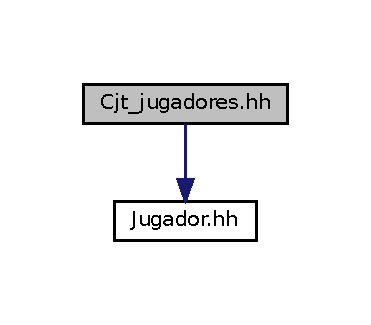
\includegraphics[width=178pt]{_cjt__jugadores_8hh__incl}
\end{center}
\end{figure}
\subsection*{Clases}
\begin{DoxyCompactItemize}
\item 
class \hyperlink{class_cjt__jugadores}{Cjt\+\_\+jugadores}
\begin{DoxyCompactList}\small\item\em Representa el conjunto de jugadores. \end{DoxyCompactList}\end{DoxyCompactItemize}


\subsection{Descripción detallada}
Especificación de la clase \hyperlink{class_cjt__jugadores}{Cjt\+\_\+jugadores}. 


\hypertarget{_cjt__torneos_8hh}{}\section{Referencia del Archivo Cjt\+\_\+torneos.\+hh}
\label{_cjt__torneos_8hh}\index{Cjt\+\_\+torneos.\+hh@{Cjt\+\_\+torneos.\+hh}}


Especificación de la clase \hyperlink{class_cjt__torneos}{Cjt\+\_\+torneos}.  


Dependencia gráfica adjunta para Cjt\+\_\+torneos.\+hh\+:\nopagebreak
\begin{figure}[H]
\begin{center}
\leavevmode
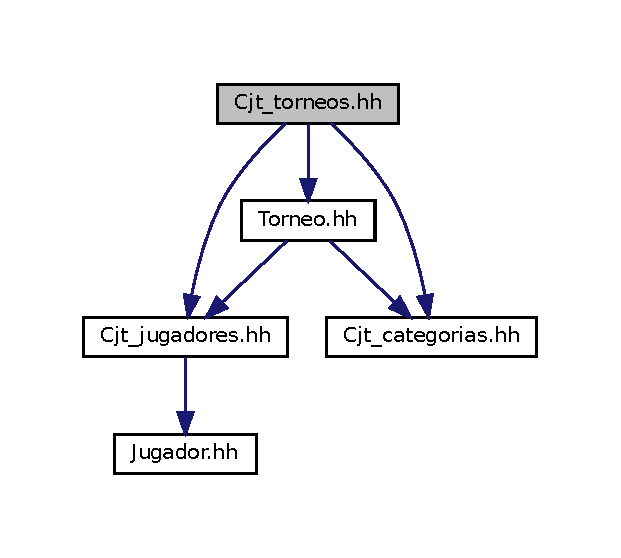
\includegraphics[width=298pt]{_cjt__torneos_8hh__incl}
\end{center}
\end{figure}
\subsection*{Clases}
\begin{DoxyCompactItemize}
\item 
class \hyperlink{class_cjt__torneos}{Cjt\+\_\+torneos}
\begin{DoxyCompactList}\small\item\em Representa el conjunto de torneos. \end{DoxyCompactList}\end{DoxyCompactItemize}


\subsection{Descripción detallada}
Especificación de la clase \hyperlink{class_cjt__torneos}{Cjt\+\_\+torneos}. 


\hypertarget{_jugador_8hh}{}\section{Referencia del Archivo Jugador.\+hh}
\label{_jugador_8hh}\index{Jugador.\+hh@{Jugador.\+hh}}


Especificación de la clase \hyperlink{class_jugador}{Jugador}.  


\subsection*{Clases}
\begin{DoxyCompactItemize}
\item 
class \hyperlink{class_jugador}{Jugador}
\begin{DoxyCompactList}\small\item\em Representa un jugador del cicuito. \end{DoxyCompactList}\end{DoxyCompactItemize}


\subsection{Descripción detallada}
Especificación de la clase \hyperlink{class_jugador}{Jugador}. 


\hypertarget{main_8cc}{}\section{Referencia del Archivo main.\+cc}
\label{main_8cc}\index{main.\+cc@{main.\+cc}}


Programa principal para la práctica.  


Dependencia gráfica adjunta para main.\+cc\+:\nopagebreak
\begin{figure}[H]
\begin{center}
\leavevmode
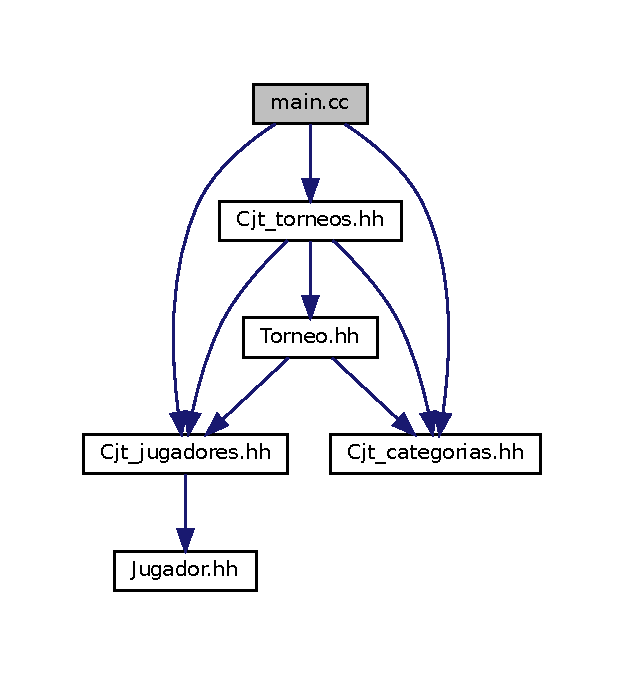
\includegraphics[width=300pt]{main_8cc__incl}
\end{center}
\end{figure}
\subsection*{Funciones}
\begin{DoxyCompactItemize}
\item 
int \hyperlink{main_8cc_ae66f6b31b5ad750f1fe042a706a4e3d4}{main} ()
\end{DoxyCompactItemize}


\subsection{Descripción detallada}
Programa principal para la práctica. 



\subsection{Documentación de las funciones}
\mbox{\Hypertarget{main_8cc_ae66f6b31b5ad750f1fe042a706a4e3d4}\label{main_8cc_ae66f6b31b5ad750f1fe042a706a4e3d4}} 
\index{main.\+cc@{main.\+cc}!main@{main}}
\index{main@{main}!main.\+cc@{main.\+cc}}
\subsubsection{\texorpdfstring{main()}{main()}}
{\footnotesize\ttfamily int main (\begin{DoxyParamCaption}{ }\end{DoxyParamCaption})}



Definición en la línea 20 del archivo main.\+cc.


\begin{DoxyCode}
20            \{
21     \hyperlink{class_cjt__categorias}{Cjt\_categorias} cat;
22     \hyperlink{class_cjt__jugadores}{Cjt\_jugadores} jug;
23     \hyperlink{class_cjt__torneos}{Cjt\_torneos} tor;
24     cat.\hyperlink{class_cjt__categorias_a25f0264b46b1c1de5af074bfae1ee5ed}{leer}();
25     tor.\hyperlink{class_cjt__torneos_af0f18e3971687674b58d020689fa2203}{leer}();
26     jug.\hyperlink{class_cjt__jugadores_a625e1ba48fc2f9b7c868820e1dc417f1}{leer}();
27     \textcolor{keywordtype}{string} operacion;
28     cin >> operacion;
29     \textcolor{keywordflow}{while} ( operacion != \textcolor{stringliteral}{"fin"}) \{
30         \textcolor{keywordflow}{if} (operacion == \textcolor{stringliteral}{"nuevo jugador"} or operacion == \textcolor{stringliteral}{"nj"}) \{
31             \textcolor{keywordtype}{string} nj;
32             cin >> nj;
33             \textcolor{keywordflow}{if} ( jug.\hyperlink{class_cjt__jugadores_a90a090845d242dd1f7dddf2d19467592}{existe}(nj)) \{
34                 cout << \textcolor{stringliteral}{"error, el jugador "} << nj 
35                      << \textcolor{stringliteral}{" ya pertenece al circuito"} << endl;
36             \}
37             \textcolor{keywordflow}{else} \{
38                 jug.\hyperlink{class_cjt__jugadores_a99640dbf83c833ed484d1bc31a36ede1}{nuevo\_jugador}(nj);
39             \}
40         \}
41         \textcolor{keywordflow}{else} \textcolor{keywordflow}{if} (operacion == \textcolor{stringliteral}{"nuevo torneo"} or operacion == \textcolor{stringliteral}{"nt"}) \{
42             \textcolor{keywordtype}{string} nt;
43             \textcolor{keywordtype}{int} c;
44             cin >> nt;
45             cin >> c;
46             \textcolor{keywordflow}{if} ( c < 1 or c > cat.\hyperlink{class_cjt__categorias_a8d99bf913eb3aaf562e5a086faaae517}{num\_categorias}()) \{
47                 cout << \textcolor{stringliteral}{"no existe la categoria "} << c  << endl; 
48             \}
49             \textcolor{keywordflow}{else} \textcolor{keywordflow}{if} (tor.\hyperlink{class_cjt__torneos_a1c36520142bc446e3f0b2fb9701246c2}{existe}(nt)) \{
50                 cout <<  \textcolor{stringliteral}{"error, el torneo "} << nt 
51                      << \textcolor{stringliteral}{" ya pertenece al circuito"} << endl;
52             \}
53             \textcolor{keywordflow}{else}\{
54                 tor.\hyperlink{class_cjt__torneos_a8e0f1049c3d772d63b3aefd885677ee3}{nuevo\_torneo}(nt,c);
55             \}
56         \}
57         \textcolor{keywordflow}{else} \textcolor{keywordflow}{if} (operacion == \textcolor{stringliteral}{"baja jugador"} or operacion == \textcolor{stringliteral}{"bj"}) \{
58             \textcolor{keywordtype}{string} nj;
59             cin >> nj;
60             \textcolor{keywordflow}{if} ( not jug.\hyperlink{class_cjt__jugadores_a90a090845d242dd1f7dddf2d19467592}{existe}(nj)) \{
61                 cout << \textcolor{stringliteral}{"error, el jugador "} << nj 
62                      << \textcolor{stringliteral}{" no existe"} << endl;
63             \}
64             \textcolor{keywordflow}{else} \{
65                 jug.\hyperlink{class_cjt__jugadores_ac0783e7a2a952975cd339f69cb040b30}{eliminar\_jugador}(nj);
66                 jug.\hyperlink{class_cjt__jugadores_a4951d7691e67c44415fdcb3119dd4148}{num\_jugadores}();
67             \}
68         \}
69         \textcolor{keywordflow}{else} \textcolor{keywordflow}{if} (operacion == \textcolor{stringliteral}{"baja torneo"} or operacion == \textcolor{stringliteral}{"bt"}) \{
70             \textcolor{keywordtype}{string} nt;
71             cin >> nt;
72             \textcolor{keywordflow}{if} ( not tor.\hyperlink{class_cjt__torneos_a1c36520142bc446e3f0b2fb9701246c2}{existe}(nt)) \{
73                 cout << \textcolor{stringliteral}{"error, el torneo "} << nt 
74                      << \textcolor{stringliteral}{" no pertenece al circuito"} << endl;
75             \}
76             \textcolor{keywordflow}{else} \{
77                 tor.\hyperlink{class_cjt__torneos_aa4a23ce93b31fe6c29b9b3a1fee2393a}{eliminar\_torneo}(nt);
78                 tor.\hyperlink{class_cjt__torneos_aba6d57df308bdbfa173578c108e19b82}{num\_torneos}();
79             \}
80         \}
81         \textcolor{keywordflow}{else} \textcolor{keywordflow}{if} (operacion == \textcolor{stringliteral}{"iniciar torneo"} or operacion == \textcolor{stringliteral}{"it"})\{
82             \textcolor{keywordtype}{string} nt;
83             cin >> nt;
84             \textcolor{keywordflow}{if} ( not tor.\hyperlink{class_cjt__torneos_a1c36520142bc446e3f0b2fb9701246c2}{existe}(nt)) \{
85                 cout << \textcolor{stringliteral}{"error, el torneo "} << nt 
86                      << \textcolor{stringliteral}{" no se puede iniciar porque no existe"} << endl; 
87             \}
88             \textcolor{keywordflow}{else} \{
89                 \textcolor{keywordtype}{int} num\_jugadores;
90                 cin >> num\_jugadores;
91                 tor.\hyperlink{class_cjt__torneos_a6b77c538bd9a25a0ec6563849736e6d6}{iniciar\_torneo}( nt, num\_jugadores);
92             \}
93         \}
94         \textcolor{keywordflow}{else} \textcolor{keywordflow}{if} (operacion == \textcolor{stringliteral}{"finalizar torneo"} or operacion == \textcolor{stringliteral}{"ft"})\{
95             \textcolor{keywordtype}{string} nt;
96             cin >> nt;
97             \textcolor{keywordflow}{if} ( not tor.\hyperlink{class_cjt__torneos_a1c36520142bc446e3f0b2fb9701246c2}{existe}(nt))\{
98                  cout << \textcolor{stringliteral}{"Error, el torneo "} << nt 
99                      << \textcolor{stringliteral}{" no se puede finalizar porque no existe"} << endl;
100 
101             \}
102             \textcolor{keywordflow}{else} \textcolor{keywordflow}{if}( not tor.\hyperlink{class_cjt__torneos_a5ba68f778eee8e1050a7f0916755dfa0}{comenzado}(nt))\{
103                 cout << \textcolor{stringliteral}{"El torneo "} << nt << \textcolor{stringliteral}{" no ha comenzado"} << endl;
104             \}
105             \textcolor{keywordflow}{else} \{
106                 tor.\hyperlink{class_cjt__torneos_aa61972563342ca00b87a3c9b0ea78b6c}{resultados\_torneo}(nt);
107             \}
108 
109         \}
110         \textcolor{keywordflow}{else} \textcolor{keywordflow}{if} (operacion == \textcolor{stringliteral}{"listar ranking"} or operacion == \textcolor{stringliteral}{"lr"})\{
111             jug.\hyperlink{class_cjt__jugadores_a2eca08ea3674049547e6eb6242da1df5}{imprimir\_ranking}();
112         \}
113         \textcolor{keywordflow}{else} \textcolor{keywordflow}{if} (operacion == \textcolor{stringliteral}{"listar jugadores"} or operacion == \textcolor{stringliteral}{"lj"})\{
114             jug.\hyperlink{class_cjt__jugadores_aeeb65f2beec6cac01abf0135b37dd104}{imprimir\_lista\_jugadores}();
115         \}
116         \textcolor{keywordflow}{else} \textcolor{keywordflow}{if} (operacion == \textcolor{stringliteral}{"listar torneos"} or operacion == \textcolor{stringliteral}{"lt"})\{
117             tor.\hyperlink{class_cjt__torneos_aeaa059c6509b254de82f218f09ff9e3e}{imprimir\_lista\_torneos}();
118         \}
119         \textcolor{keywordflow}{else} \textcolor{keywordflow}{if} (operacion == \textcolor{stringliteral}{"listar categorias"} or operacion == \textcolor{stringliteral}{"lc"})\{
120             cat.\hyperlink{class_cjt__categorias_acd18a2fe2b4336dd5faa7e418962d713}{imprimir\_categorias}();
121         \}
122     \}
123 \}
\end{DoxyCode}

\hypertarget{_torneo_8hh}{}\section{Referencia del Archivo Torneo.\+hh}
\label{_torneo_8hh}\index{Torneo.\+hh@{Torneo.\+hh}}


Especificación de la clase \hyperlink{class_torneo}{Torneo}.  


Dependencia gráfica adjunta para Torneo.\+hh\+:\nopagebreak
\begin{figure}[H]
\begin{center}
\leavevmode
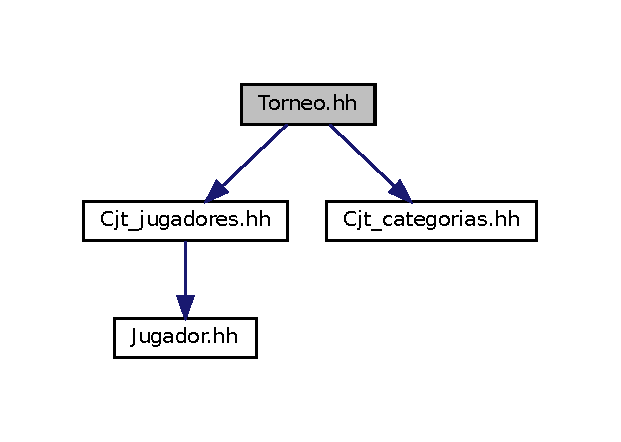
\includegraphics[width=298pt]{_torneo_8hh__incl}
\end{center}
\end{figure}
\subsection*{Clases}
\begin{DoxyCompactItemize}
\item 
class \hyperlink{class_torneo}{Torneo}
\begin{DoxyCompactList}\small\item\em Representa un torneo del circuito. \end{DoxyCompactList}\end{DoxyCompactItemize}


\subsection{Descripción detallada}
Especificación de la clase \hyperlink{class_torneo}{Torneo}. 


%--- End generated contents ---

% Index
\backmatter
\newpage
\phantomsection
\clearemptydoublepage
\addcontentsline{toc}{chapter}{Índice}
\printindex

\end{document}
